\clearpage
\section{重积分}
\setstretch{1.75}

\subsection{复习要点}

\subsubsection{重积分概念与性质提要}

本章开头概括了重积分的定义方法，即类似于一元函数定积分“分割、近似、求和、取极限”的步骤.
对于具体的严格定义则不必细究，只需知道与计算有关的性质即可.
接下来以二重积分为例总结：

(1)~常数可以提到积分号之外；

(2)~积分对函数的可加性；

(3)~积分对区域的可加性；

(4)~积分不等式：若在区域$D$上有不等式$f(x,y) \le g(x,y)$，则：
\begin{eq1}
    \iint_{D} f(x,y) ~\d \sigma \le \iint_{D} g(x,y) ~\d \sigma
\end{eq1}

(5)~积分绝对值不等式：
\begin{eq1}
    \left| \iint_{D} f(x,y) ~\d \sigma \right| \le
    \iint_{D} | f(x,y) | ~\d \sigma
\end{eq1}

(6)~积分中值定理：若函数$f(x,y)$在有界闭区域$D$上连续，
则在$D$上至少存在一点$(x_0,y_0)$，使：
\begin{eq1}
    \iint_{D} f(x,y) ~\d \sigma = f(x_0,y_0) \cdot S
\end{eq1}
其中$S$是区域$D$的面积.\vspace{1em}

在讨论重积分的计算之前，
我们再解释几个概念上的问题（仍然以二重积分为例）：\par
1.~重积分的定义涉及到将区域$D$分割成一系列子区域$D_i$，
正如一元函数定积分中将定义域区间分割成一系列子区间.
那么，每个子区间$D_i$的面积$\Delta \sigma_i$要怎么定义呢？
如果按照高数中所学，用积分来计算面积，就犯了循环定义的错误；
而且退一步说，区域边界也未必能表示成可积函数的形式.
所以，必须在这里引入另一种更加普适的“面积”（\textbf{测度}）定义来作为积分的基础.
这已经超出了高数课程的要求. \par
2.~关于二元函数可积性的条件，教材中指出，
有界闭区域上（分片）连续的二元函数是可积的.
如果将闭区域改为开区域，则不一定成立，例如在开区域$D = \left \{ (x,y)~|~ x^2 + y^2 < 1 \right \}$内，
二元函数$f(x,y) = \frac{1}{1 - \sqrt{x^2 + y^2}}$是连续函数，但不可积.
不过，如果已经给了一个有界闭区域上的（分片）连续函数，再挖去区域内“面积”为$0$的一些点（例如去掉区域边界使其变为开区域），则不影响可积性.\par
3.~在做重积分计算题时，我们是通过\textbf{累次积分}来计算的.
简单来说是先固定$x$（或$y$），对$y$（或$x$）做定积分，再对$x$（或$y$）做定积分.
在高数课程中，我们不需要怀疑重积分和累次积分会不会有区别，直接算就完事了.
不过事实上，这个怀疑是可以有的.
因为累次积分之于重积分的关系正如\textbf{累次极限}之于\textbf{全面极限}.
这里举出一个二元函数可积但累次极限不存在的例子，感兴趣的同学可以自行研究.
设$D = [0,1] \times [0,1]$，当$(x,y) \in D$时，令：
\[
f(x,y) =
\begin{cases}
    \frac{1}{k} &\quad x = \frac{1}{k}~(k \in \mathbb{N}), ~y \in \mathbb{Q} \\
    0 &\quad \text{其他}
\end{cases}
\]

\subsubsection{直角坐标系下的计算}

\textbf{1.~~二重积分化累次积分} \vspace{0.25em}

若积分区域$D$是“$X$型区域”（图$1$左），
可以采取“先$y$后$x$”的策略，
即转化为如下的累次积分（后两式是同一累次积分的不同书写方法，
今后统一用后者）：
\begin{eq1}
    \iint_{D}f(x,y) ~\d x \d y =
    \int_{a}^{b} \left[  \int_{\varphi_{1}(x)}^{\varphi_{2}(x)} f(x,y) ~\d y \right] ~\d x =
    \int_{a}^{b} ~\d x \int_{\varphi_{1}(x)}^{\varphi_{2}(x)} f(x,y) ~\d y
\end{eq1}

若积分区域$D$是“$Y$型区域”（图$1$右），可以采取“先$x$后$y$”的策略，
即转化为如下的累次积分：
\begin{eq1}
    \iint_{D}f(x,y) ~\d x \d y =
    \int_{c}^{d} ~\d y \int_{\psi_{1}(x)}^{\psi_{2}(x)} f(x,y) ~\d x
\end{eq1}

\begin{figure}[H]
    \centering
    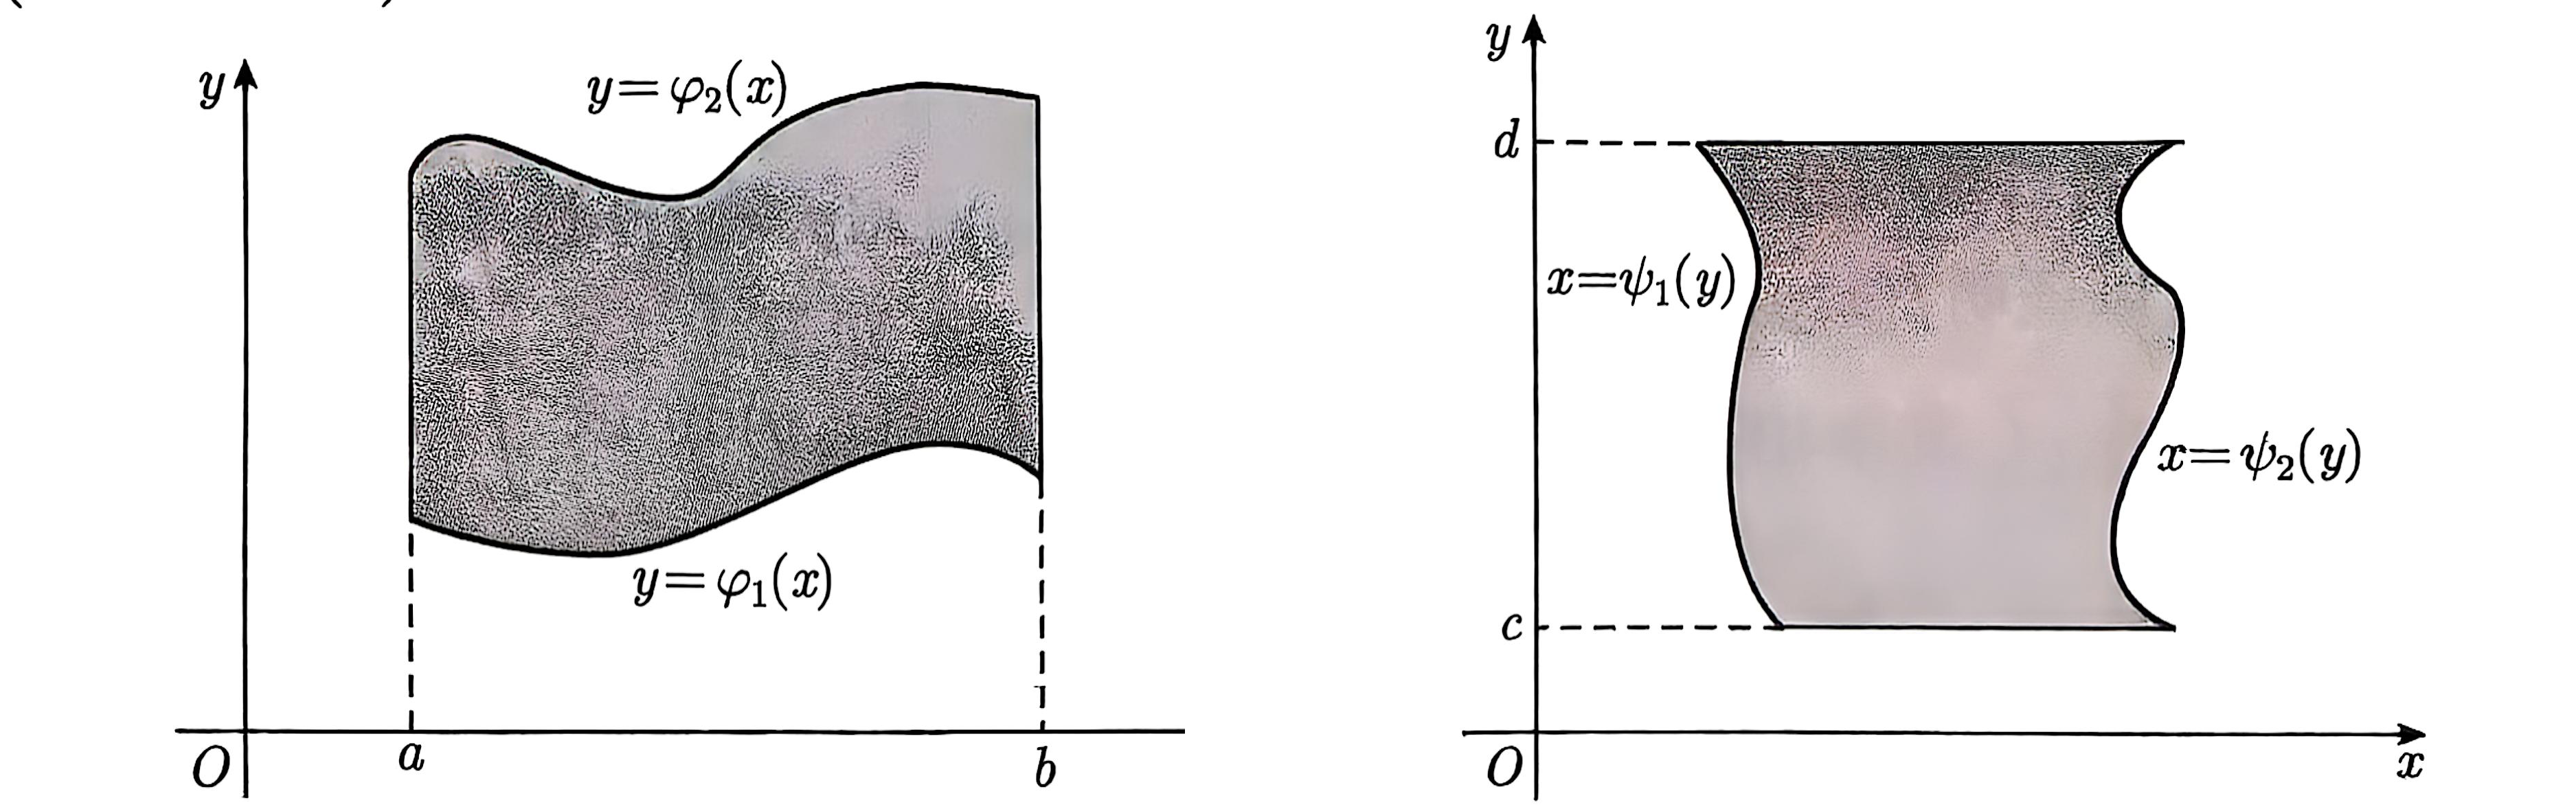
\includegraphics[width=0.8\textwidth]{fig7_1.png}
    \caption{$X$型区域与$Y$型区域}
\end{figure}

需要注意，虽然一元函数的定积分允许积分下限大于上限，
但是将二重积分转化为累次积分时，有$\varphi_{1}(x) \le \varphi_{2}(x)$
（或$\psi_{1}(x) \le \psi_{2}(x)$）的要求.
例如，设$D$是$\sin x$的图像与$x$轴围成的区域（图2）.
要将$D$上对$f(x,y)$的二重积分写成累次积分，不可以这样写：
$$
\iint_{D} f(x,y)~\d x\d y
= \int_{0}^{2\pi} ~\d x \int_{0}^{\sin x} f(x,y)~\d y
$$\par
这是因为当$\pi < x < 2 \pi$时（即对于子区域$D_2$），$\sin x < 0$，此时对$y$的积分上下限应该反过来.
也就是说，$D_1$与$D_2$需要分开来写.
正确的写法是：
\begin{equation}
    \begin{aligned}
    \iint_{D} f(x,y)~\d x\d y
    &= \iint_{D_1} f(x,y)~\d x\d y + \iint_{D_2} f(x,y)~\d x\d y \\
    &= \int_{0}^{\pi} ~\d x \int_{0}^{\sin x} f(x,y)~\d y
    + \int_{\pi}^{2\pi} ~\d x \int_{\sin x }^{0} f(x,y)~\d y
        \nonumber
    \end{aligned}
\end{equation}

\begin{figure}[H]
    \centering
    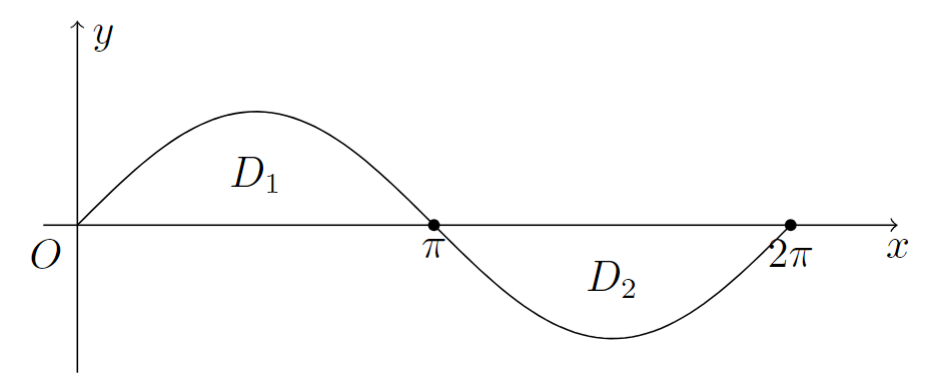
\includegraphics[width=0.6\textwidth]{fig7_2.png}
    \caption{$\sin x$图像与$x$轴围成的区域}
\end{figure}

\textbf{2.~~三重积化累次积分} \vspace{0.25em}

在三重积分中，一般用$\Omega$来标记积分区域.
注意此时的“积分区域”$\Omega$是指一个立体图形，而非平面区域了.

若$\Omega$是曲顶/曲底柱体（以图3左的情形为例），可以采取“先一后二”的策略，即先固定$x$和$y$,对$z$做定积分，再对$x$和$y$在投影区域$D$内做二重积分：
$$
\iiint_{\Omega} f(x,y,z)~\d x \d y \d z=
\iint_{D} ~\d x \d y \int_{z_{1}(x,y)}^{z_{2}(x,y)} f(x,y,z)~\d z
$$\par
若$\Omega$介于两平行平面之间（以图3右的情形为例），可以采取“先二后一”的策略，即先固定$z$，取$\Omega$的水平截面$D_z$，在其上对$x$和$y$做二重积分，之后再对$z$做定积分.
注意当$z$变化时，截面$D_z$也会变化：
$$
\iiint_{\Omega} f(x,y,z)~\d x \d y \d z=
\int_{a}^{b} ~\d z \iint_{D_z} f(x,y,z)~\d x \d y
$$

\begin{figure}[H]
    \centering
    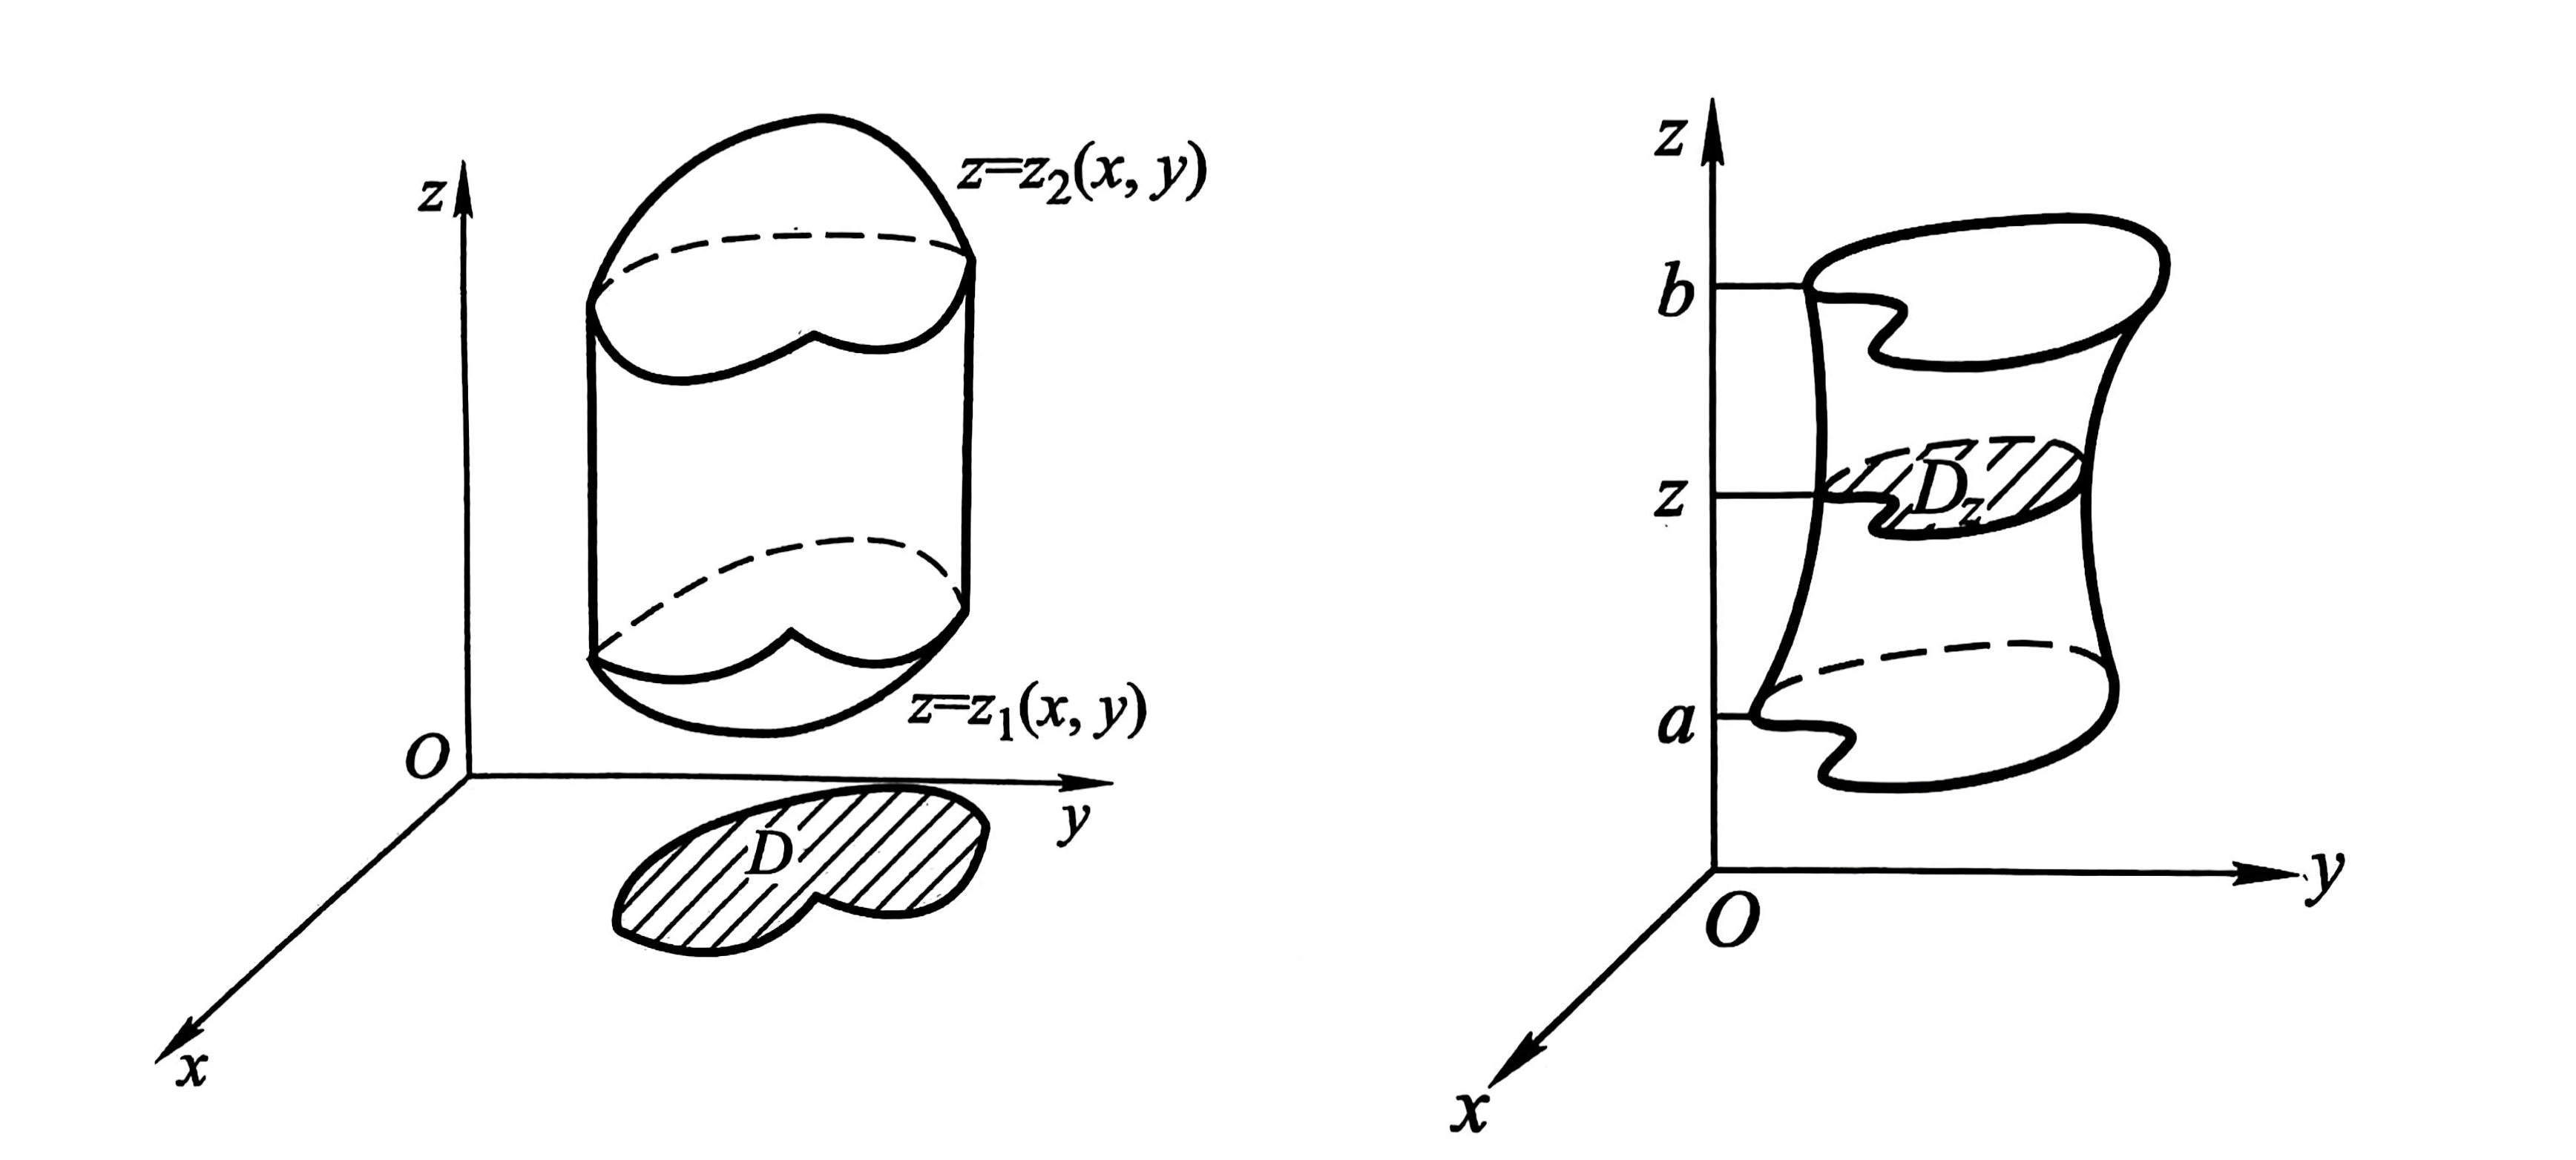
\includegraphics[width=0.75\textwidth]{fig7_3.png}
    \caption{三重积分的典型积分区域}
\end{figure}

\textbf{3.~~利用重积分的对称性}

利用好积分区域和被积函数的对称性，可以大大缩短计算时间.
尤其要注意的是对称区域上
\textbf{奇函数}的对称性.
若二元函数$f(x,y)$\textbf{关于$y$是奇函数}，
而积分区域$D$关于$x$轴对称（图4左）；
或者，$f(x,y)$\textbf{关于$x$是奇函数}，
而积分区域$D$关于$y$轴对称（图4右），两种情况下都有：
\begin{eq1}
    \iint_{D} f(x,y)~\d x \d y = 0
\end{eq1}

这提示我们，如果在对称区域上积分，而被积函数中含有相应奇函数的项，可以干脆划去不算.
对于高度对称的积分区域（如正方形区域、圆形区域），更应该对奇函数敏感，不能容忍它在计算式里出现.

\begin{figure}[H]
    \centering
    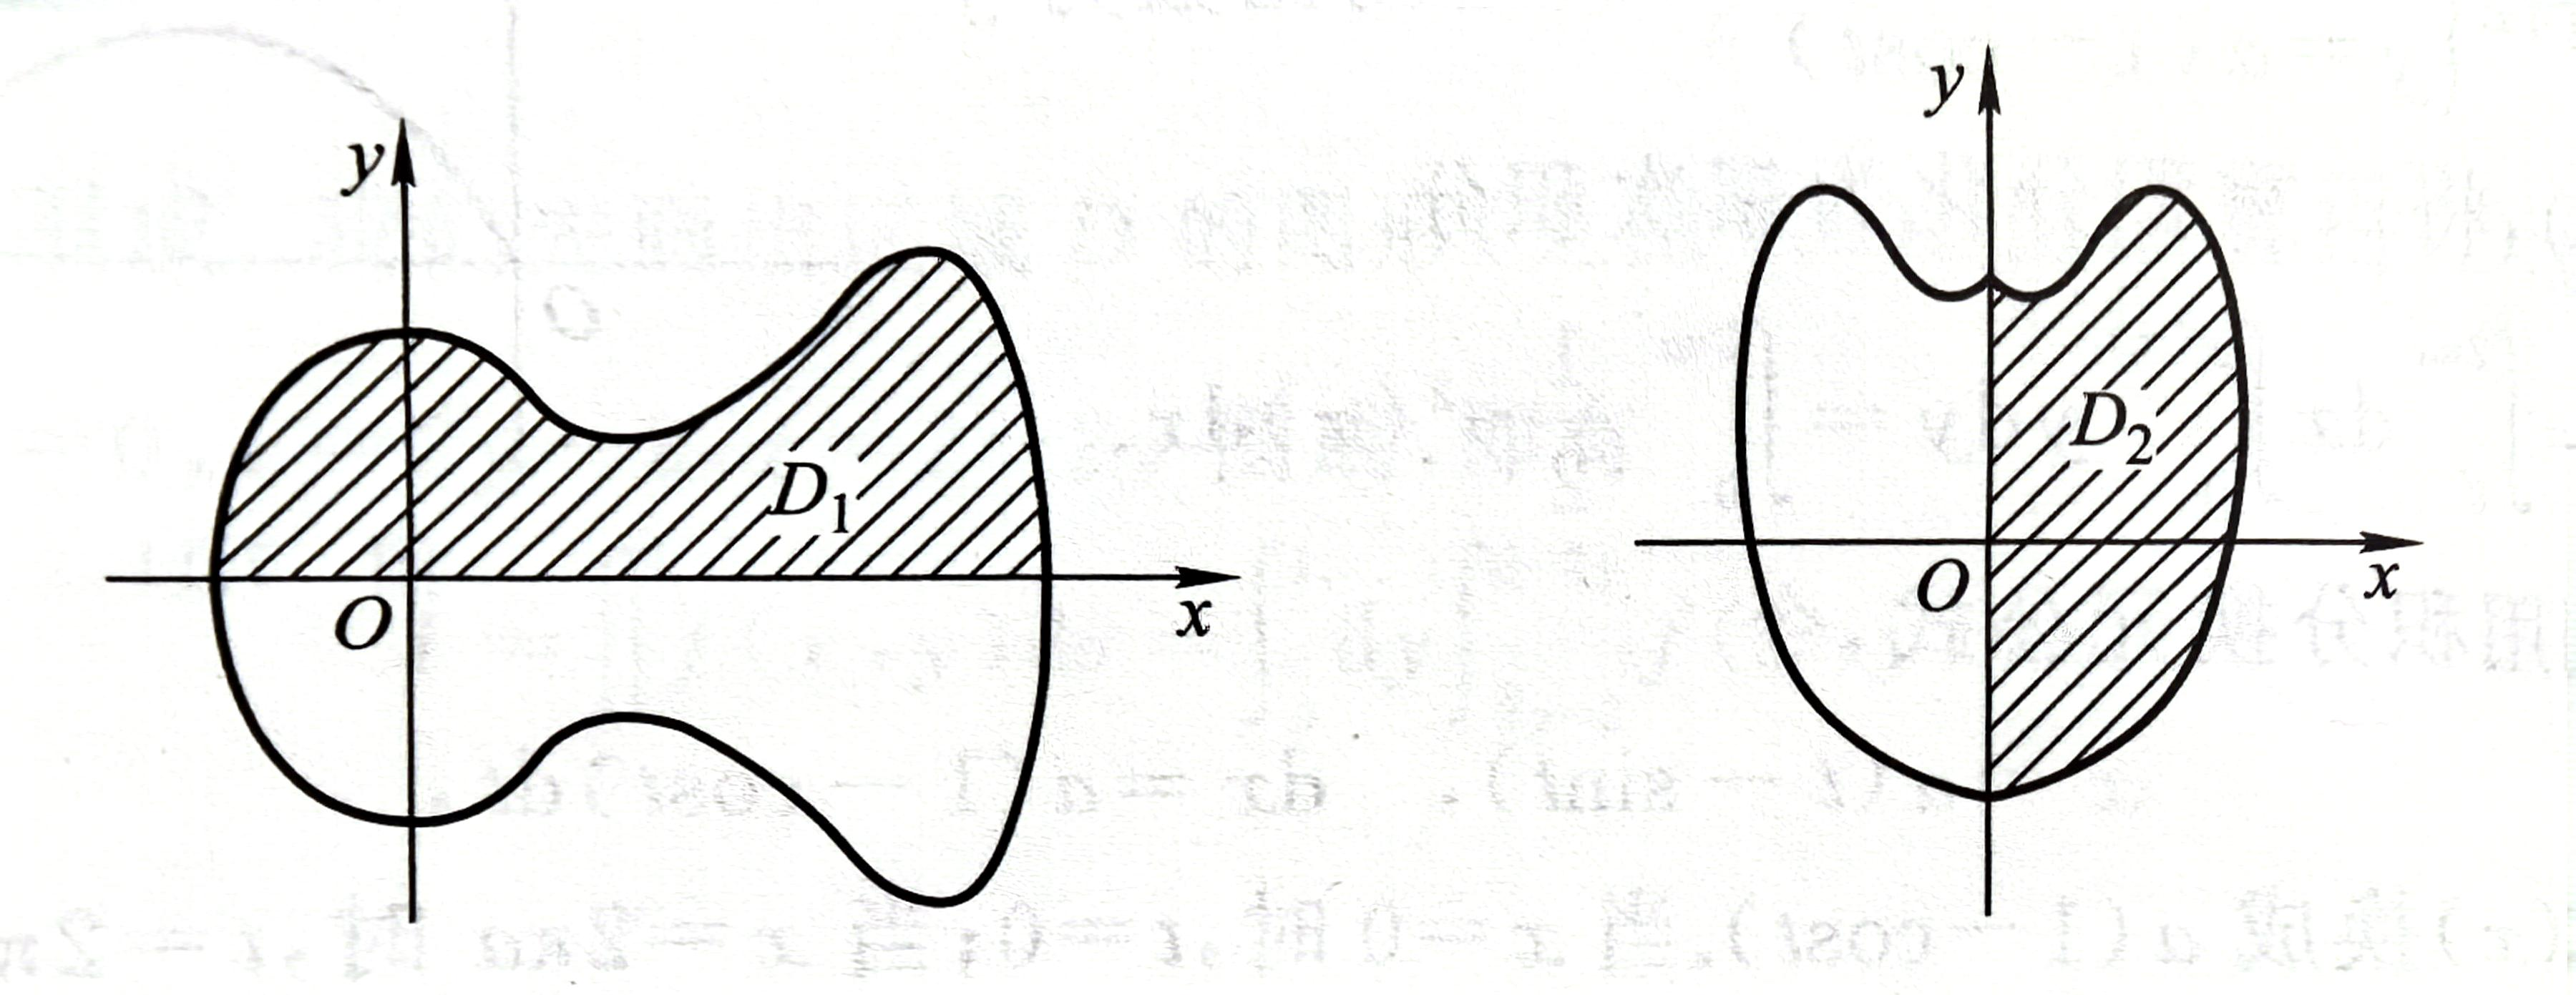
\includegraphics[width=0.75\textwidth]{fig7_4.png}
    \caption{对称的积分区域（记积分区域整体为$D$）}
\end{figure}

\subsubsection{换元法}\par
换元法的易错点在于容易忘记乘雅可比行列式的绝对值$|J|$.
以二重积分为例.
若要将变量$(x,y)$换为$(u,v)$，两组变量之间的关系由两个二元函数$x = x(u,v)$，$y = y(u,v)$确定.
则变换前后的面积微元$\d \sigma = \d x \d y$与$\d \sigma ' = \d u \d v$
有如下关系：
\begin{eq1}
\d x \d y = |J| ~\d u \d v
\end{eq1}
其中$J$即为\textbf{雅可比行列式}，其定义为：
\begin{eq1}
    J = \frac{D(x,y)}{D(u,v)} =
    \begin{vmatrix}
        \frac{\partial x}{\partial u} & \frac{\partial x}{\partial v} \vspace{1.5ex}  \\
        \frac{\partial y}{\partial u} & \frac{\partial y}{\partial v}
    \end{vmatrix}
\end{eq1}

如果完整地写到二重积分式中，应该长这样（设变换前后的积分区域分别是$D$和$D'$，被积函数是$f$）：
\begin{eq1}
    \iint_{D} f(x,y) ~\d x \d y = \iint_{D'} f(x(u,v),y(u,v))~ |J| ~\d u \d v
\end{eq1}

注意，$J$是指雅可比行列式，$|J|$才是雅可比行列式的绝对值.
关于雅可比行列式的推导可以不用掌握，只需要理解其意义.
从形式上讲，这相当于在一元函数积分的换元法中利用一阶微分的形式不变性（设$x = x(u)$）：
\begin{eq1}
    \d x = \frac{\d x}{\d u} \cdot \d u = x'(u) ~\d u
\end{eq1}\par

从几何意义上讲，换元这一操作使得原来的积分区域$D$映射到了新变量下的积分区域$D'$.
在变换中积分区域发生了“扭曲”，区域面积也会变化（图5）.
雅可比行列式$J$在每点处的值就等于该点附近区域面积被“伸缩”的比例.
因为面积不能为负数，所以需要给$J$加上绝对值.

\begin{figure}[H]
    \centering
    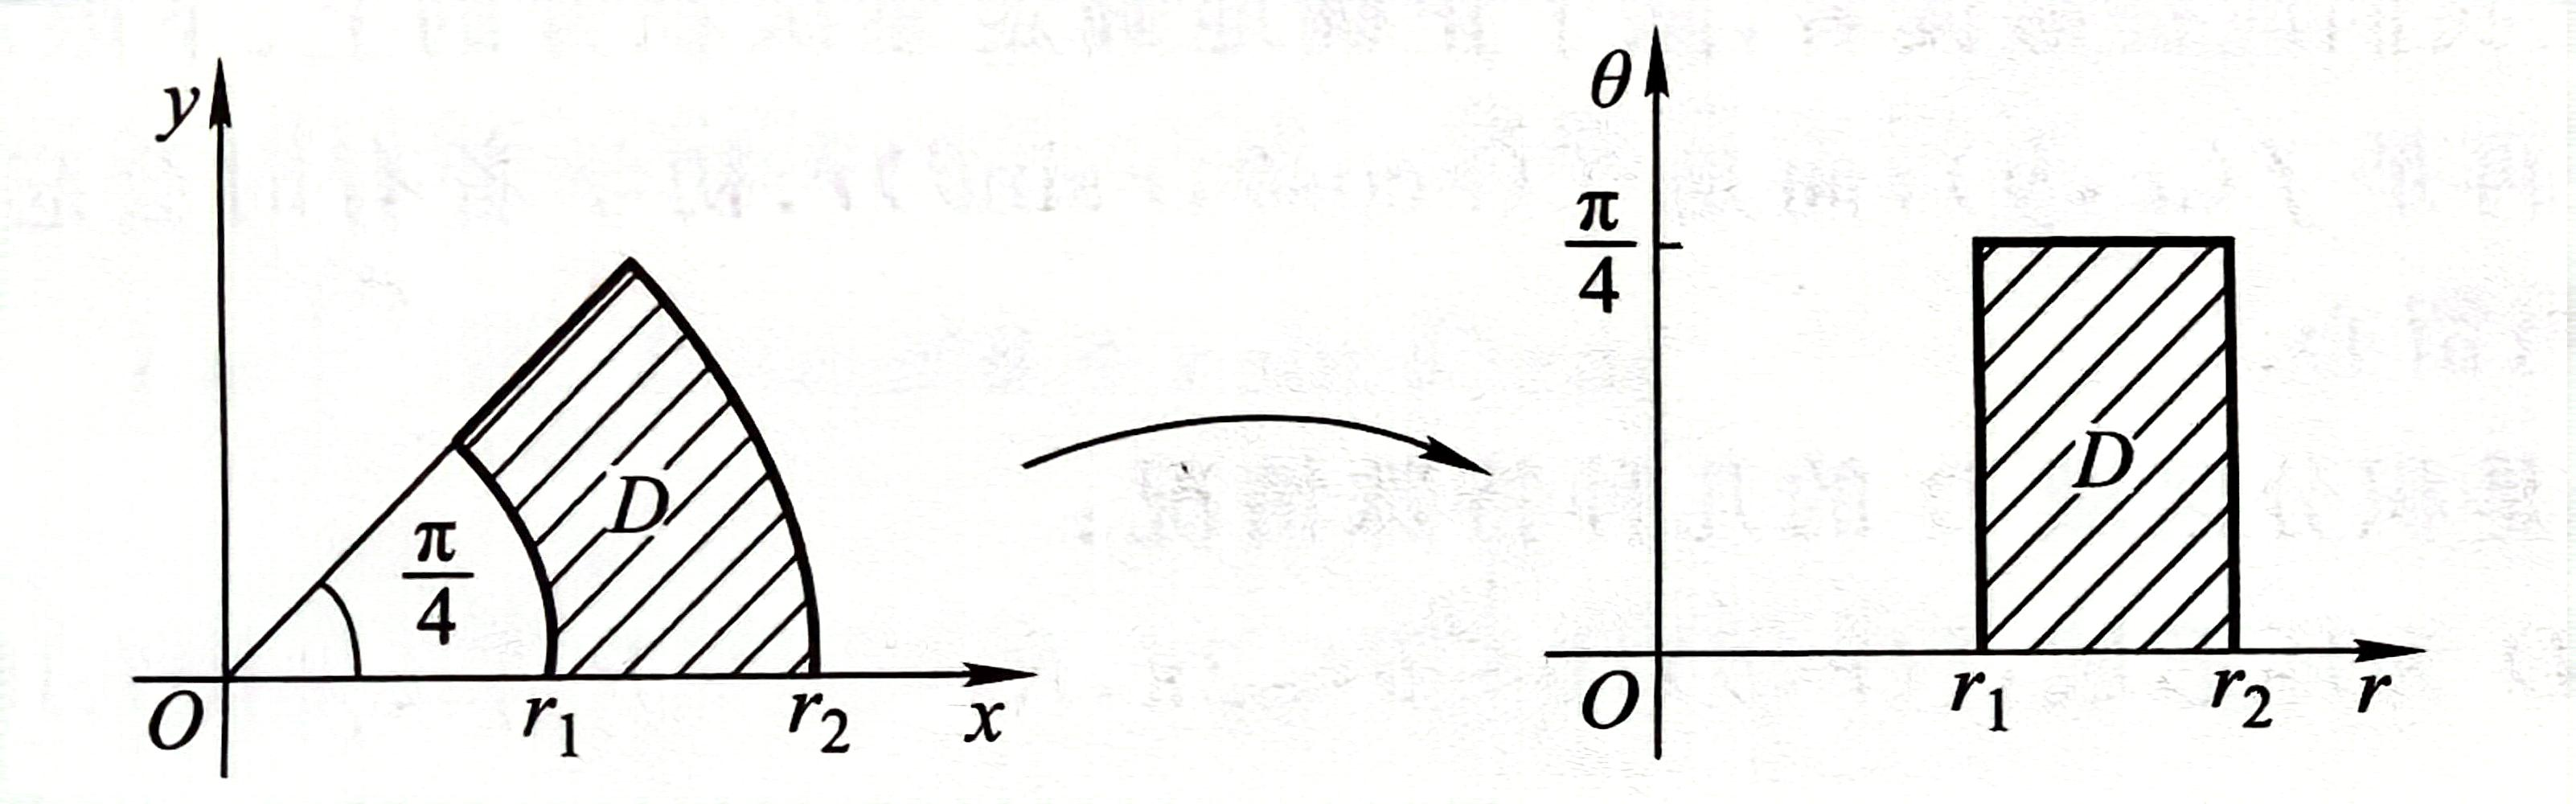
\includegraphics[width=0.75\textwidth]{fig7_5.png}
    \caption{极坐标换元下积分区域发生的“扭曲”}
\end{figure}

对于三重积分的换元$(x,y,z) \mapsto (u,v,w)$，雅可比行列式则可以写为：
\begin{eq1}
    J = \frac{D(x,y,z)}{D(u,v,w)} =
    \begin{vmatrix}
        \frac{\partial x}{\partial u} & \frac{\partial x}{\partial v} & \frac{\partial x}{\partial w} \vspace{1.5ex}  \\
        \frac{\partial y}{\partial u} & \frac{\partial y}{\partial v} & \frac{\partial y}{\partial w} \vspace{1.5ex} \\
        \frac{\partial z}{\partial u} & \frac{\partial z}{\partial v} & \frac{\partial z}{\partial w} \vspace{1.5ex}
    \end{vmatrix}
\end{eq1}

实际上可以按照这个规律写出任意$n$阶的雅可比行列式，但是一般不会用到.
最后，课本上介绍了三种常用的换元法，下面列出公式.
这些换元下的雅可比行列式可以用特殊的几何法推导出来，不过同样不需要掌握.

(1)~二重积分的（广义）极坐标变换：
\begin{eq1}
    \setstretch{1.25}
    \begin{cases}
        x = r \cos  \theta \\
        y = r \sin \theta
    \end{cases} \Rightarrow
    \d x \d y = r ~\d r \d \theta ~~~~~~~
    \begin{cases}
        x = ar \cos \theta  \\
        y = br \sin \theta
    \end{cases} \Rightarrow
    \d x \d y = abr ~\d r \d \theta
\end{eq1}

\setstretch{1.75}

(2)~三重积分的柱坐标变换：
\begin{eq1}
   \setstretch{1.25}
    \begin{cases}
        x = r \cos \theta  \\
        y = r \sin \theta  \\
        z = z
    \end{cases}  \Rightarrow
    \d x \d y d z= r ~\d r \d \theta \d z
\end{eq1}

\setstretch{1.75}

(3)~三重积分的（广义）球坐标变换
 （提示：需要注意区分$\varphi$和$\theta$的几何意义，前者是“竖直方向夹角”，后者是“水平方向夹角”. 有些书中会将两个字母反过来使用.）：
\begin{eq1}
    \setstretch{1.25}
    \begin{cases}
        x = \rho \sin \varphi \cos \theta  \\
        y = \rho \sin \varphi \sin \theta  \\
        z = \rho \cos \varphi
    \end{cases}  \Rightarrow
    \d x \d y d z= \rho^2 \sin \varphi ~\d \rho \d \varphi \d \theta
\end{eq1}

$$
\setstretch{1.25}
 \begin{cases}
        x = a \rho \sin \varphi \cos \theta  \\
        y = b \rho \sin \varphi \sin \theta  \\
        z = c \rho \cos \varphi
    \end{cases}  \Rightarrow
    \d x \d y d z= abc \rho^2 \sin \varphi ~\d \rho \d \varphi \d \theta
$$
\setstretch{1.75}

\subsubsection{*一元函数定积分和多重积分的区别}

同学们可能会想，一元函数定积分的换元法是否为多重积分换元法的特殊情况？
但实践下来却发现不是如此.
设一元函数$f(x)$定义在区间$I = [a,b]$上.
考虑一个最简单的变量替换$x = -u$，变换后的区间$I' = [-b,-a]$.\par
如果根据多重积分换元法的理论来计算，此时需要计算一阶雅可比行列式$J = \frac{\d x}{\d u} = -1$，再取绝对值$|J| = 1$.
因而有：
\begin{eq1}
    f(x) ~\d x =  f(-u) \cdot \left| \frac{\d x}{\d u} \right| \cdot \d u  = f(-u) \cdot 1 \cdot \d u
\end{eq1}

但事实上，我们对一元函数换元时，应利用一阶微分的形式不变性，得到：
\begin{eq1}
    f(x) ~\d x = f(-u) \cdot \frac{\d x}{\d u} \cdot \d u = f(-u) \cdot (-1) \cdot ~\d u
\end{eq1}

二者相差一个负号.
其中的区别在于一元函数定积分的换元当中是不给$J = \frac{\d x}{\d u}$加绝对值的.
这是为什么呢？
实际上，我们对一元函数定积分和多重积分的定义有一个重大的区别.
例如在二重积分中，我们只要说“$f(x,y)$在区域$D$上的二重积分”，就不会有任何歧义.
但是在一元函数定积分中，说“$f(x)$在区间$I$上的定积分”则是模糊不清的，因为这既可能指
$\int_{a}^{b} f(x) ~\d x$，也可能指$\int_{b}^{a} f(x) ~\d x$，二者是一正一负的关系.
换句话说，一元函数定积分的“区间”有正向和负向之分，而多重积分的“积分区域”则不存在正负的说法.
这也是为什么将重积分转化为累次积分时必须要求积分下限小于积分上限.\par

刚才的讨论涉及到的数学概念是坐标系的\textbf{定向}.
事实上对于任何$n$维的欧氏坐标系都可以指定两种不同的定向：
对$1$维而言，可以指定为$x$轴的正向和负向；对$2$维而言，可以指定为坐标平面的法向量朝上或者朝下；对$3$维而言，则是左手和右手.
显然，本章所学的多重积分是不考虑积分区域的定向的.
但是在之后要学的某些类型的曲线积分和曲面积分中，则需要考虑不同的定向带来的正负之分.
不妨从本章开始就对有无定向的区别敏感起来.

\subsubsection{重积分的几何应用}
(1)~计算平面区域的面积：设平面区域为$D$，则其面积$S_D$可用二重积分表示：
\begin{eq1}
    S_D = \iint_{D} 1 ~\d \sigma
\end{eq1}

(2)~计算空间区域的体积：设空间区域为$\Omega$，则其体积$V_{\Omega}$可用三重积分表示：
\begin{eq1}
    V_{\Omega} = \iiint_{\Omega} 1 ~\d V
\end{eq1}

(3)~计算空间曲面的（表）面积：

第一种情况，若空间曲面$S$的方程是二元函数$z =f (x,y)$，曲面在$xOy$平面上的投影区域（即$(x,y)$的范围）是$D$.
则曲面$S$的面积公式：
\begin{eq1}
    S = \iint_{D} ~d S = \iint_{D} \sqrt{1 + f_{x}^{2}(x,y) + f_{y}^{2}(x,y)} ~\d \sigma
\end{eq1}
其中$\d S = \sqrt{1 + f_{x}^{2}(x,y) + f_{y}^{2}(x,y)} ~\d \sigma$是\textbf{空间曲面$S$的面积微元}.\par
第二种情况，曲面$S$是由参数方程给出：
$$
    \setstretch{1.25}
    \begin{cases}
        x = x(u,v) \\
        y = y(u,v) \\
        z = z(u,v)
    \end{cases}
    ~~~(u,v) \in D'
$$ \par
\setstretch{1.75}
设三个基本量$E$、$F$和$G$分别为：
$$
\setstretch{1.25}
    \begin{cases}
        E = \bm{r}_u \cdot \bm{r}_u = x_u^2 + y_u^2 + z_u^2 \\
        F = \bm{r}_u \cdot \bm{r}_v = x_u x_v +y_u y_v + z_u z_v\\
        G = \bm{r}_v \cdot \bm{r}_v = x_v^2 + y_v^2 + z_v^2
    \end{cases}
$$
\setstretch{1.75}
\par
则曲面$S$的面积公式：
\begin{eq1}
    S = \iint_{D} ~d S = \iint_{D} \sqrt{EG - F^2} ~\d u \d v
\end{eq1}
其中$\d S = \sqrt{EG-F^2} ~\d u \d v$是\textbf{空间曲面$S$的面积微元}.
这里提到的两个面积微元的公式十分深刻而且重要，应当熟记，之后在计算\textbf{第一型曲面积分}时还会继续使用.
公式的推导可以不必掌握，但是要理解其过程中利用曲面法向量对面积微元进行“投影”的思路.\par
本章最后还列举了重积分的物理应用：(1)~求物体质量；(2)~求物体质心；(3)~求物体绕轴的转动惯量，以及绕定点的转动惯量.
这些在高数中不会考，但是在普通物理中会考.

\subsection{解题方法}

\subsubsection{利用对称性简化计算}

奇函数在对称区域内的积分值为$0$.
这条性质在考试中必须时刻想起来使用.
有些积分如果展开来写会出现很多项，
很有可能其中某几项是奇函数，积分值为$0$，可以直接从积分中去掉.
这样看似复杂的积分可能也会变得简单.
如果不看对称性的话，要么很快就被大串的式子吓退，要么在根本不必要的步骤上浪费很多时间，在计算量大的考试中会很吃亏.

\begin{example}
\label{ex:ch07-01}
计算$\iint_{D} \left( \sin^3 x \cos y + x^6 y^3 \right) \d \sigma$.
其中$D:~x^2 + y^2 \le R^2$.
\end{example}

\begin{solution}
$\sin^3 x \cos y$是关于$x$的奇函数，$x^6 y^3$是关于$y$的奇函数.
积分区域$D$关于$x$轴和$y$轴都对称.
故积分值为$0$.
\end{solution}

\begin{example}
\label{ex:ch07-02}
计算$\iint_{D} x \left( 1 + y \sqrt{x^2 + y^2} \right) ~\d \sigma$.
区域$D$由$y=x$，$y=1$，$x = -1$围成.
\end{example}

\begin{analysis}
这题若直接做会比较耗费精力，有没有进一步化简的方法？
须发现被积函数关于$x$是奇函数，关于$y$也有部分是奇函数.
积分区域$D$虽然整体不是关于坐标轴对称，但是好在形状比较规整，
可以切割出一些对称区域来.
\end{analysis}

\begin{solution}
将积分区域$D$进行分割（图6）.
则原积分化为：
\begin{eq1}
    \iint_{D} x \left( 1 + y \sqrt{x^2 + y^2} \right) ~\d \sigma
    &=
    \iint_{D_1 \cup D_2} x \left( 1 + y \sqrt{x^2 + y^2} \right) ~\d \sigma
    \\&~~+
    \iint_{D_3 \cup D_4} x \left( 1 + y \sqrt{x^2 + y^2} \right) ~\d \sigma
\end{eq1}

\begin{figure}[H]
    \centering
    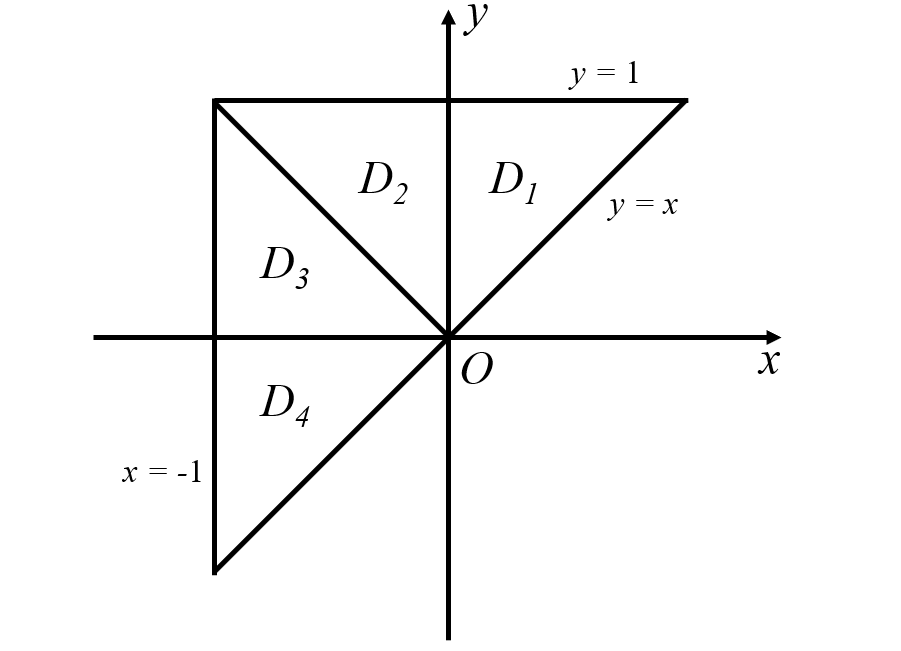
\includegraphics[width=0.4\textwidth]{fig7-6.png}
    \caption{例\ref{ex:ch07-02}积分区域}
\end{figure}

其中，区域$D_1$和$D_2$关于$y$轴对称，
且被积函数为关于$x$的奇函数.
故$D_1 \cup D_2$上的积分为$0$，即：
\begin{eq1}
    \iint_{D} x \left( 1 + y \sqrt{x^2 + y^2} \right) ~\d \sigma
    &=
    \iint_{D_1 \cup D_2}  \left( x + xy \sqrt{x^2 + y^2} \right) ~\d \sigma
\end{eq1}

另外，$xy \sqrt{x^2 + y^2}$是关于$y$的奇函数，剩下的一项$x$关于$y$是偶函数.
而区域$D_3$和$D_4$关于$x$轴对称.
故积分可以进一步化简为：
\begin{eq1}
    \iint_{D} x \left( 1 + y \sqrt{x^2 + y^2} \right) ~\d \sigma
    &=
    \iint_{D_3 \cup D_4}  x ~\d \sigma
    &=
    2 \iint_{D_3} x ~ \d \sigma
\end{eq1}

化为累次积分并计算：
\begin{eq1}
    2 \iint_{D_3} x ~ \d \sigma
    &=
    2 \int_{-1}^{0} ~\d x \int_{0}^{-x} x ~\d y\\
    &= 2 \int_{-1}^{0} (-x^2)  ~\d x \\
    &= -\frac{2}{3}
\end{eq1}
\end{solution}

\begin{example}[2023]
\label{ex:ch07-03}
计算积分

\[
I = \iint _ { D } ( x + y + x y ) ^ { 2 } \mathrm { ~ d } \sigma
\]

其中 $D = \left\{ ( x , y ) \in \mathbb { R } ^ { 2 } \mid x ^ { 2 } + y ^ { 2 } \le 1 \right\} .$
\end{example}

\begin{analysis}
平方和展开有$6$项之多.
若直接用极坐标换元，式子将会很长.
但事实上，平方和展开中的交叉项要么是$x$的奇函数，要么是$y$的奇函数.
而积分区域又是非常对称的.
因此只需计算平方项即可.
\end{analysis}

\begin{solution}
将被积函数展开并利用对称性：
\begin{eq1}
    I &= \iint_{D} \left( x^2 + y^2 + x^2y^2 + 2xy + 2x^2y + 2xy^2 \right) ~\d \sigma \\
    &= \iint_{D} \left( x^2 + y^2 + x^2y^2 \right) ~\d \sigma
\end{eq1}

采用极坐标换元：
\begin{eq1}
    I &=
    \int_0^{2\pi} \int_0^1
    \left( r^2 + r^4\cos^2\theta\sin^2\theta \right) r\,\mathrm{d}r\,\mathrm{d}\theta\\
    &=
    \int_0^{2\pi} \int_0^1
    \left( r^3 + \frac{1}{4} \cdot r^5 \sin^2 2\theta \right) \,\mathrm{d}r\,\mathrm{d}\theta\\
    &=
    \int_0^1 ~\d r  \int_0^{2\pi}
    \left( r^3 + \frac{1}{4} \cdot r^5 \cdot \frac{1- \cos 4\theta}{2} \right) ~\d \theta \\
\end{eq1}

对$\theta$积分时，利用三角函数在一个周期内的积分为$0$：
\begin{eq1}
    I &=
    2 \pi \int_0^1 \left( r^3 + \frac{r^5}{8} \right) ~\d r \\
    &= \frac{13 \pi }{24}
\end{eq1}
\end{solution}

（注：在上题中，如果一开始没有注意到对称性，全部代入三角换元，
在后续对$\theta$做积分时，
也可以利用三角函数在一个周期内的积分为$0$来消去一些具有对称性的项.
这种对于三角函数的积分技巧也是计算中常用的.）\par \vspace{1em}

我们现在再介绍一种利用对称性的技巧：
若积分区域$D$关于$y=x$对称，则其上的二重积分满足轮换对称性，即$x$与$y$可以互换位置，
积分值不变：
\begin{eq1}
    \iint_{D} f(x,y)~\d \sigma =
    \iint_{D} f(y,x)~\d \sigma
\end{eq1}

仅仅交换$x$与$y$不足以解决什么问题.
但是可以把两个积分组合起来：
\begin{eq1}
    \iint_{D} f(x,y)~\d \sigma =
    \frac{1}{2} \iint_{D} \left(f(x,y)+f(y,x)\right)~\d \sigma
\end{eq1}

如果$f(x,y)+f(y,x)$的形式很简单，就可以考虑使用轮换对称性进行组合积分.

\begin{example}
\label{ex:ch07-04}
计算二重积分
$\iint _ {D}  x(1-y^3) + y(1+x^3) ~\d x \d y$，
其中$D$为
$x^2 + y^2 \le 2x+2y$.
\end{example}

\begin{solution}
积分区域是以$(1,1)$为圆心，$\sqrt{2}$为半径的圆，
关于$y=x$对称.
由轮换对称性：
\begin{eq1}
    \iint _ {D}  f(x,y) ~\d x \d y
    &= \frac{1}{2} \iint _ {D}  f(x,y) + f(y,x)~\d x \d y \\
    &= \frac{1}{2} \iint _ {D} x(1-y^3) + y(1+x^3) + y(1-x^3) + x(1+y^3) ~\d x \d y \\
    &= \iint_{D} x+y ~\d x \d y \\
    &= 4 \pi
\end{eq1}
\end{solution}

\begin{example}
\label{ex:ch07-05}
计算积分
$I = \iint_{D} \frac{a \sqrt{x+1} + b \sqrt{y+1}}{\sqrt{x+1} + \sqrt{y+1}} ~\d \sigma$.
其中区域$D$为$x^2 + y^2 \le 1$，$x\ge 0$，$y \ge 0$.
\end{example}

\begin{solution}
积分区域$D$关于$y=x$对称，故可以利用轮换对称性：
\begin{eq1}
    \iint _ {D}  f(x,y) ~\d x \d y
    &= \frac{1}{2} \iint _ {D}  f(x,y) + f(y,x)~\d x \d y \\
    &= \frac{1}{2} \iint_{D} \frac{a \sqrt{x+1} + b \sqrt{y+1}}{\sqrt{x+1} + \sqrt{y+1}} +
    \frac{a \sqrt{y+1} + b \sqrt{x+1}}{\sqrt{y+1} + \sqrt{x+1}} ~\d \sigma \\
    &= \frac{1}{2} \iint_{D} a+b ~\d \sigma \\
    &= \frac{(a+b)\pi}{8}
\end{eq1}
\end{solution}

\subsubsection{选择合适的坐标系（换元法）}

如果积分在直角坐标系下难以解决，首先要考虑是否应该换元.
一个理想的换元应该既让积分区域变得简单，也让被积函数的表达式变得简单.
但有时二者可能无法兼得.
这种情况下一般需要先照顾积分区域.
因为：(1)出题人可能故意把被积函数设计得很复杂以增加计算量，不容易通过换元化简；
(2)累次积分中的上下限取决于积分区域的表示方法，而上下限的表达式最终会融入到外层积分的表达式中.
因此被积函数形式简单也不一定就方便计算.

积分区域的形状是对换元方法的绝佳提示.
例如，圆形的积分区域（二重积分）十有八九要用极坐标，
圆柱形的积分区域（三重积分）一般要用柱坐标.
如果是复杂得“不可名状”的积分区域，也不用慌张，可以自由选择换元的方式把较复杂的表达式替换掉.
需要注意不要忘记计算雅可比行列式，也不要忘记给雅可比行列式取绝对值.

\begin{example}
\label{ex:ch07-06}
计算二重积分
$\iint _ { \Omega } \left( x ^ { 2 } + y ^ { 2 } \right) \d x \d y$，
其中$\Omega$为椭圆：
$\frac { x ^ { 2 } } { a ^ { 2 } }
+ \frac { y ^ { 2 } } { b ^ { 2 } } \le 1 $.
\end{example}

\begin{solution}
采用广义极坐标变换
$x = ar\cos\theta$, $y = br\sin\theta$.
其中 $r \in [0, 1]$，
$\theta \in [0, 2\pi)$.
雅可比行列式$J = abr$.
则原积分化为：
\begin{eq1}
    \iint_{\Omega'} \left(x^2 + y^2\right) \mathrm{d}x\,\mathrm{d}y
    = \int_0^{2\pi} \int_0^1 r^2(a^2\cos^2\theta + b^2\sin^2\theta) \cdot abr\,\mathrm{d}r\,\mathrm{d}\theta
\end{eq1}

整理后得到：
\begin{eq1}
    \iint_{\Omega'} \left(x^2 + y^2\right) \mathrm{d}x\,\mathrm{d}y
    = ab \int_0^{2\pi} \int_0^1 r^3(a^2\cos^2\theta + b^2\sin^2\theta)\,\mathrm{d}r\,\mathrm{d}\theta
\end{eq1}

先对$r$积分得到：
\begin{eq1}
    \iint_{\Omega'} \left(x^2 + y^2\right) \mathrm{d}x\,\mathrm{d}y
    = ab \cdot \frac{1}{4} \int_0^{2\pi} \left(a^2\cos^2\theta + b^2\sin^2\theta\right) \, \mathrm{d}\theta
\end{eq1}

再对$\theta$积分.
利用三角恒等式$\cos^2\theta = \frac{1 + \cos{2\theta}}{2}$和
$\sin^2\theta = \frac{1 - \cos{2\theta}}{2}$.
再考虑到$\cos{2\theta}$的周期性和对称性，
它在$0$到$2 \pi$上的积分为$0$.
由此得到：
\begin{eq1}
    \iint_{\Omega'} \left(x^2 + y^2\right) \mathrm{d}x\,\mathrm{d}y
    &=
    ab \cdot \frac{1}{4} \int_0^{2\pi}
    \left(a^2 \cdot \frac{1 + \cos{2\theta}}{2} + b^2 \cdot \frac{1 - \cos{2\theta}}{2}\right) \, \mathrm{d}\theta \\
    &=
    ab \cdot \frac{1}{4} \int_0^{2\pi}
    \left(\frac{a^2}{2} + \frac{b^2}{2} \right) \, \mathrm{d}\theta \\
    &= \frac{ab(a^2 + b^2) \pi }{4}
\end{eq1}
\end{solution}

\begin{example}
\label{ex:ch07-07}
计算$\iint_{D} (x+y) ~\d \sigma $，
其中$D$由$x^2 + y^2 \le 2x+2y$所确定.
\end{example}

\begin{analysis}
积分区域是圆域$(x-1)^2 + (y-1)^2 \le 2$.
可将其“平移”到以原点为圆心，这样既使积分区域变得简单，也能利用上被积函数的对称性.
\end{analysis}

\begin{solution}
令$u = x-1$，$v=y-1$.
则变换后的积分区域$D'$为$u^2 + v^2 \le 2$.
计算雅可比行列式：
\begin{eq1}
    J =
    \begin{vmatrix}
        \frac{\partial x}{\partial u} & \frac{\partial x}{\partial v} \\[4pt]
        \frac{\partial y}{\partial u} & \frac{\partial y}{\partial v}
    \end{vmatrix}
    =
    \begin{vmatrix}
        1 & 0 \\[-4pt]
        0 & 1
    \end{vmatrix}
    = 1
\end{eq1}

则原积分化为：
\begin{eq1}
    \iint_{D} (x+y) \, \mathrm{d}\sigma
    = \iint_{D'} (u + v + 2) \cdot |J| \, \mathrm{d}u \, \mathrm{d}v
    = \iint_{D'} (u + v + 2) \, \mathrm{d}u \, \mathrm{d}v.
\end{eq1}

注意$u$和$v$在对称区域$D'$内是各自的奇函数，故积分值为0.
除去$u+v$之后，被积函数只剩下了$2$，积分值应等于区域$D'$的面积的$2$倍，
即$4 \pi $.
\end{solution}

\setstretch{2.25}

\begin{example}[2023]
\label{ex:ch07-08}
计算积分
$I = \iiint _ { \Omega } \frac { ( x + y + z ) ^ { 2 } \sqrt { 1 + x ^ { 2 } + y ^ { 2 } } }
{ \left( x ^ { 2 } + y ^ { 2 } + z ^ { 2 } \right) \left( 1 + x ^ { 2 } + y ^ { 2 } + z ^ { 2 } \right) }
 \d V ,$
其中 $\d V$ 即 $\d x \d y \d z$，$\Omega$
是由曲面
$z = \sqrt{1 + x^{2} + y^{2}}$，
$z = \sqrt{3\left(1 + x^{2} + y^{2}\right)}$和
$x^{2} + y^{2} = 1$ 所围成的区域.

\setstretch{1.75}
\end{example}

\begin{analysis}
积分区域是在柱面$x^2 + y^2 =1$的基础上加盖了“圆顶”和“圆底”，从积分区域来看采用柱坐标最合适.
在看到被积函数的时候可能会犹豫一下，因为分子上的$(x+y+z)^2$在柱坐标下似乎比较复杂.
但是不要忘记先应用对称性！
积分区域关于$xOz$平面和$yOz$平面对称，
故展开后的交叉项$2xy+2yz+2zx$积分值为$0$，只需要考虑平方项的积分即可.
\end{analysis}

\begin{solution}
将分子上的平方和展开：
\begin{eq1}
    (x+y+z)^2 = x^2 + y^2 + z^2 + 2xy+2yz+2zx
\end{eq1}

其中，$2xy$、$2yz$、$2zx$要么是$x$的奇函数，要么是$y$的奇函数.
而积分区域关于$xOz$平面和$yOz$平面对称.
故利用对称性化简：
\begin{eq1}
    I &=
    \iiint _ { \Omega } \frac { ( x^2 + y^2 + z^2 ) \sqrt { 1 + x ^ { 2 } + y ^ { 2 } } }
    { \left( x ^ { 2 } + y ^ { 2 } + z ^ { 2 } \right) \left( 1 + x ^ { 2 } + y ^ { 2 } + z ^ { 2 } \right) }
    ~\d V \\
    &=
    \iiint _ { \Omega } \frac { \sqrt { 1 + x ^ { 2 } + y ^ { 2 } } }
    {  1 + x ^ { 2 } + y ^ { 2 } + z ^ { 2 }}
    ~\d V
\end{eq1}

应用柱坐标换元$x = r \cos \theta$，$y = r \sin \theta$：
\begin{align*}
    I &= \iiint_{\Omega} \frac{\sqrt{1 + r^2}}{1+r^2 + z^2} \cdot r ~\d r \d \theta \d z \\
    &= \int_0^{2 \pi}\d \theta \int_{0}^{1}\d r
    \int_{\sqrt{1+r^2}}^{\sqrt{3(1+r^2)}} \frac{r\sqrt{1 + r^2}}{1+r^2 + z^2} ~\d z \\
    &= 2\pi \int_{0}^{1}\d r
    \int_{\sqrt{1+r^2}}^{\sqrt{3(1+r^2)}} \frac{r\sqrt{1 + r^2}}{1+r^2 + z^2} ~\d z \\
    &= 2\pi \int_{0}^{1}
    \left( \arctan \frac{z}{\sqrt{1+r^2}} \right) \bigg|_{z=r \sqrt{1+r^2}}^{z=\sqrt{3(1+r^2)}} ~\d r \\
    &= 2\pi \int_{0}^{1}
    r \left( \arctan \sqrt{3} - \arctan 1 \right)  ~\d r \\
    &= \frac{\pi^2}{6} \cdot \int_0^1 r ~\d r \\
    &= \frac{\pi^2}{12}
\end{align*}
\end{solution}

\begin{example}
\label{ex:ch07-09}
计算二重积分
$\iint_{D} \frac{1}{xy}~ \d \sigma$.
其中$D:~ 2 \le \frac{x}{x^2 + y^2} \le 4,~ 2 \le \frac{y}{x^2 + y^2} \le 4$.
\end{example}

\begin{analysis}
此题虽然被积函数形式简单，但是积分区域实在无法下手.
此时只能先照顾积分区域.
\end{analysis}

\begin{solution}
令$u = \frac{x}{x^2 + y^2}$，$v = \frac{y}{x^2 + y^2}$.
变换后的积分区域$D'$为$2 \le u \le 4$，$2 \le v \le 4$.
接下来需要计算雅可比行列式$J$.
如果直接计算，需要把$x$，$y$改写成$(u,v)$的函数，比较麻烦.
这里我们利用一个结论：互为逆变换的雅可比行列式互为倒数.
直接计算$u_x,~u_y,~v_x,~v_y$，于是：
\begin{eq1}
    J^{-1}
    =
    \begin{vmatrix}
        u_x & u_y \\[-4pt]
        v_x & v_y
    \end{vmatrix}
    =
    -\frac{1}{(x^2 + y^2)^2}
\end{eq1}

则我们要的雅可比行列式的绝对值为：
\begin{eq1}
    |J| = (x^2 + y^2)^2
\end{eq1}
原积分化为：
\begin{eq1}
    \iint_{D} \frac{1}{xy} ~\d \sigma
    &= \iint_{D} \frac{(x^2 + y^2)^2}{xy} \cdot \frac{1}{(x^2 + y^2)^2} ~\d \sigma \\
    &= \iint_{D'} \frac{1}{uv} \cdot \frac{1}{(x^2 + y^2)^2} \cdot |J| ~\d u \d v \\
    &= \iint_{D'} \frac{1}{uv} ~\d u \d v \\
    &= \int_{2}^{4} \frac{1}{u} ~\d u  \int_2^4 \frac{1}{v} ~\d v \\
    &= \left( \ln 2 \right)^2
\end{eq1}
\end{solution}

\begin{example}
\label{ex:ch07-10}
设$D$是$x^2 + y^2 = 1$和$x+y=1$在第一象限所围成的区域.
计算二重积分$\iint_{D} \frac{1}{xy(\ln^2 x + \ln^2 y)}~\d x \d y$.
\end{example}

\begin{analysis}
这题我们需要照顾被积函数的形式，因为分母上的$\ln$平方不好处理.
首先用换元把对数替换掉.
后续对于积分区域的处理，也需要充分考虑被积函数本身的性质.
\end{analysis}

\begin{solution}
令$u = \ln x$，$v = \ln y$.
变换后的积分区域$D'$为$e^{2u} + e^{2v} = 1$与$e^u + e^v = 1$所围成的区域.
雅可比行列式：
\begin{eq1}
    J
    =
    \begin{vmatrix}
        x_u & x_v \\[-4pt]
        y_u & y_v
    \end{vmatrix}
    =
    e^u e^v
\end{eq1}

则原积分化为：
\begin{eq1}
    \iint_{D} \frac{1}{xy(\ln^2 x + \ln^2 y)}~\d x \d y
    &= \iint_{D'} \frac{1}{e^u e^v (u^2 + v^2 )}\cdot |J| ~\d u \d v \\
    &= \iint_{D'} \frac{1}{u^2 + v^2} ~\d u \d v
\end{eq1}

被积函数的形式让人想到可以再用极坐标换元.
令$u = r \cos \theta$，$v = r \sin \theta$，
注意变换后的积分区域$D''$.
它是由曲线$C_1:e^{r \cos \theta}+ e^{r \sin \theta} = 1$和
$C_2:e^{2r \cos \theta} + e^{2r \sin \theta} = 1$所围成的区域.
积分进行到这一步，我们一般需要开始转化成累次积分了.
这里按惯例将$\theta$作为外层积分的变量.
考虑到$u$和$v$都非正，即$\cos \theta$和$\sin \theta$都非正，
因此$\theta \in \left[ \pi, \frac{3\pi}{2} \right]$.
不过$r$的积分上下限表示出来比较复杂.
这个做法可以继续下去吗？
我们关注到被积函数的形式：

\begin{eq1}
    \iint_{D'} \frac{1}{u^2 + v^2} ~\d u \d v
    &= \iint_{D''} \frac{1}{r^2} \cdot r ~\d r \d \theta \\
    &= \int_0^{2\pi} \d \theta \int_{r_2(\theta)}^{r_1(\theta)} \frac{1}{r} ~\d r
\end{eq1}

以上我们将$r$的积分上下限分别用$r_1(\theta)$和$r_2(\theta)$暂时代替.
实际上这也是积分区域边界曲线$C_1$和$C_2$所对应的极坐标方程.
我们将看到，计算这个积分不需要完全知道$r_1(\theta)$和$r_2(\theta)$的具体表达式.
对$\frac{1}{r}$积分会得到：
\begin{eq1}
    \iint_{D'} \frac{1}{u^2 + v^2} ~\d u \d v
    &=\int_{\pi}^{3\pi / 2} \left(\ln r \bigg|_{r_2(\theta)}^{r_1(\theta)}\right) ~\d \theta   \\
    &=\int_{\pi}^{3\pi / 2} \ln \left(\frac{r_1(\theta)}{r_2(\theta)}\right) ~\d \theta
\end{eq1}

因此这个积分最后如何表示仅取决于$\frac{r_1(\theta)}{r_2(\theta)}$.
注意$C_1$和$C_2$的方程相比，$C_2$其实是用$2r$替换了$C_1$中的$r$.
因此一定有$r_1(\theta) = 2r_2(\theta)$的关系.
因此这个积分得到了极大的简化，可以立即算出：
\begin{eq1}
    \int_{\pi}^{3\pi / 2} \ln \left(\frac{r_1(\theta)}{r_2(\theta)}\right) ~\d \theta
    &= \int_{\pi}^{3\pi / 2} \ln 2 ~\d \theta \\
    &= \frac{\pi}{2} \cdot \ln 2
\end{eq1}
\end{solution}

（注：即使没有注意到$r_1(\theta)$与$r_2(\theta)$的关系，
二者的表达式也可以显式地写出来，强行做下去就能做出来，就看敢不敢了.）

\subsubsection{特殊函数重积分}
以绝对值或者$\mathop{max}$、$\mathop{max}$形式给出的函数，
积分的基本方法是对积分区域进行划分，使每个子区域内的被积函数恢复成初等函数.

\begin{example}
\label{ex:ch07-11}
$f ( x , y ) = \mathop{max} \left\{ \sqrt { x ^ { 2 } + y ^ { 2 } } , 1 \right\} , D = \{ ( x , y ) | ~| x | \le y \le 1 \} .$
    求 $\iint _ { D } f ( x , y ) \mathrm { d } \sigma $.
\end{example}

\begin{solution}
如图7所示，将 $D$ 分成三块，中间一块记为 $D _ { 3 } $，
左、右两块分别记为 $D _ { 1 }$ 与 $D _ { 2 } $，
则：
\begin{eq1}
    f ( x , y ) &= \mathop{max} \left\{ \sqrt { x ^ { 2 } + y ^ { 2 } } , 1 \right\} \\
    &=
    \begin{cases}
        \sqrt { x ^ { 2 } + y ^ { 2 } } , & ( x , y ) \in D _ { 1 } \cup D _ { 2 } , \\[-4pt]
        1 , & ( x , y ) \in D _ { 3 }
    \end{cases}
\end{eq1}

将积分拆解成$D_1 \cup D_2$和$D_3$两部分:

\begin{eq1}
    \iint _ { D } f ( x,y ) ~\mathrm { d } \sigma
    &= \iint _ { D _ { 1 } \cup D _ { 2 } } \sqrt { x ^ { 2 } + y ^ { 2 } } \mathrm { ~ d } \sigma + \iint _ { D _ { 3 } } \mathrm { ~ d } \sigma \\
    &= \int _ { \pi / 4 } ^ {3 \pi / 4 } \mathrm { ~ d } \theta \int _ { 1 } ^ { 1 / \sin \theta  } r ^ { 2 } \mathrm { ~ d } r + \frac { \pi } { 4 } \\
    &= \frac { 1 } { 3 } \int _ { \pi / 4 } ^ {3 \pi / 4 } \left( \csc ^ { 3 } \theta - 1 \right) \mathrm { d } \theta + \frac { \pi } { 4 }\\
    &= \frac { 1 } { 3 } \int _ { \pi / 4 } ^ {3 \pi / 4 } \csc ^ { 3 } \theta ~\mathrm { d } \theta + \frac { \pi } { 1 2 }
\end{eq1}

记$I = \int _ { \pi / 4 } ^ {3 \pi / 4 } \csc ^ { 3 } \theta ~\mathrm { d } \theta$，则：
\begin{eq1}
    I &= - \int _ { \pi / 4 } ^ {3 \pi / 4 } \csc \theta ~\d (\cot \theta)  \\
    &= - \csc \theta \cot \theta \bigg|_{ \pi / 4 } ^ {3 \pi / 4 } -
    \int_{ \pi / 4 } ^ {3 \pi / 4 } \cot^2 \theta \csc \theta ~\d \theta \\
    &= 2\sqrt{2} - \int_{ \pi / 4 } ^ {3 \pi / 4 }  (\csc^2 \theta -1) \csc \theta ~\d \theta \\
    &= 2\sqrt{2} - I + \int_{ \pi / 4 } ^ {3 \pi / 4 } \csc \theta ~\d \theta \\
    &= 2\sqrt{2} - I + \ln | \csc \theta - \cot \theta| \bigg|_{ \pi / 4 } ^ {3 \pi / 4 } \\
    &= 2\sqrt{2} - I + 2\ln (\sqrt{2} + 1)
\end{eq1}

故$I = \sqrt{2} + \ln(\sqrt{2} + 1)$. 则原积分的值为$\frac{\sqrt{2}}{3} + \frac{1}{3} \ln (\sqrt{2} + 1) + \frac{\pi}{12}$.
\end{solution}

\begin{figure}[H]
    \centering
    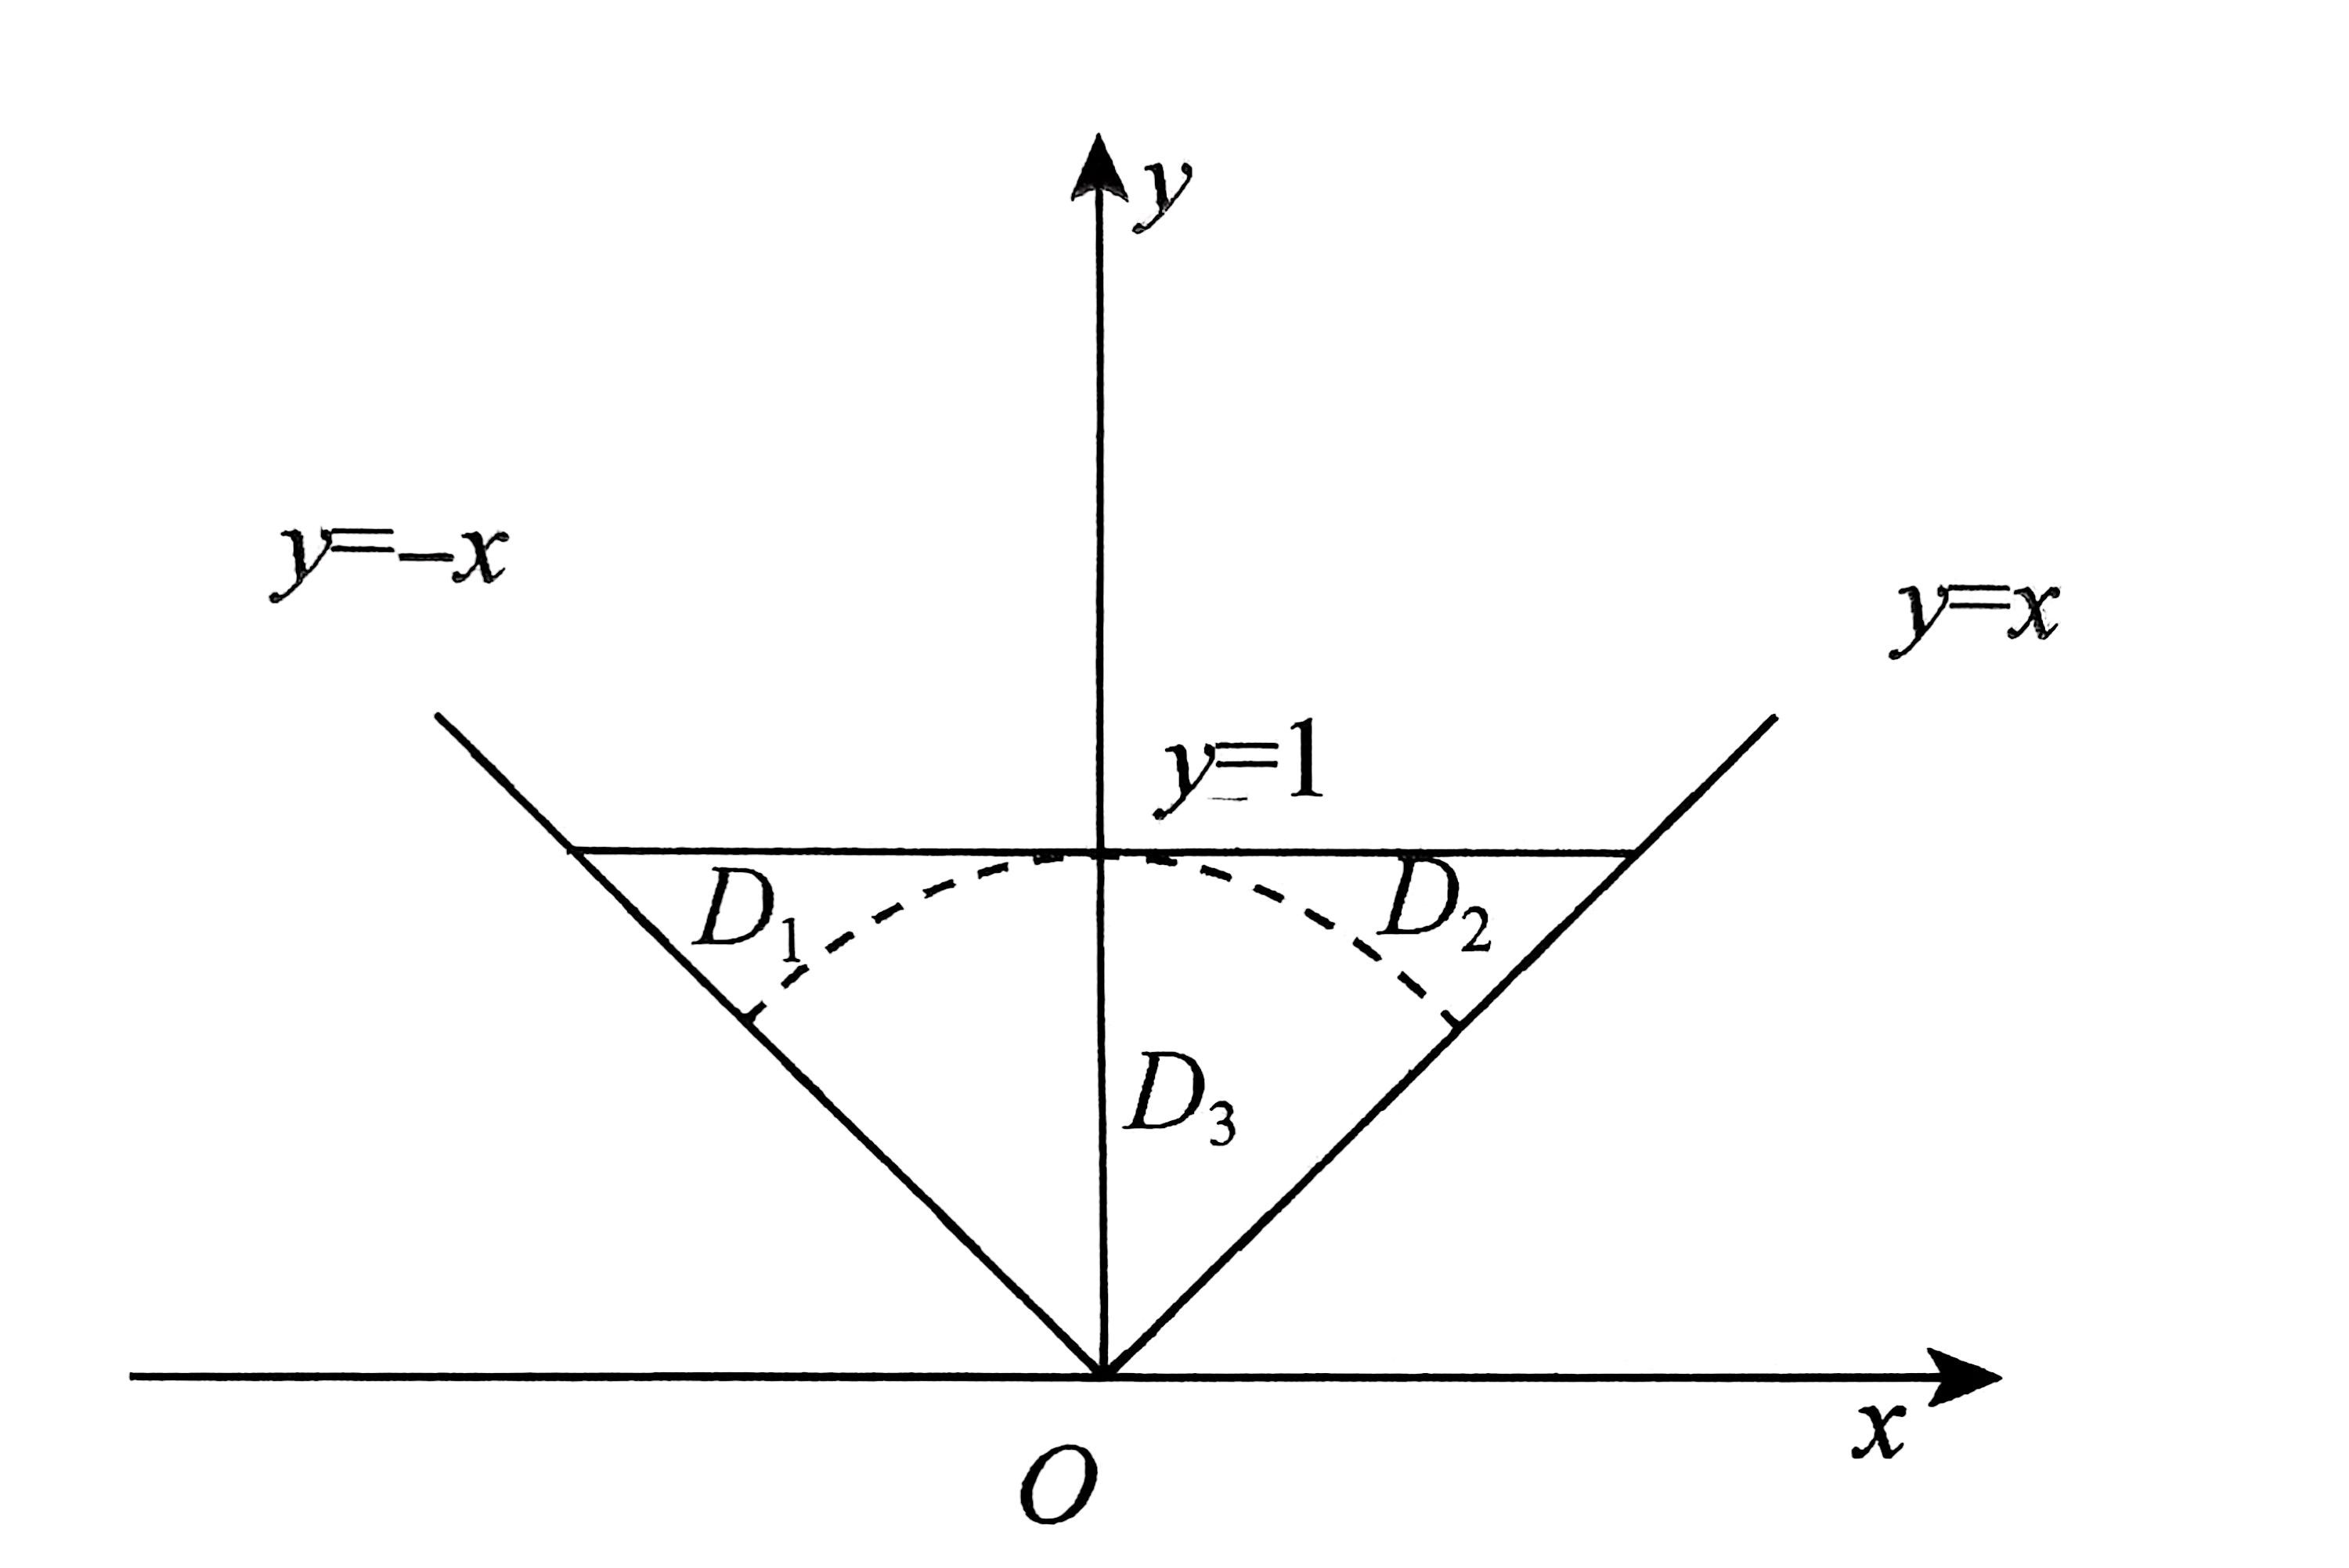
\includegraphics[width=0.4\textwidth]{fig7_7.jpg}
    \caption{例\ref{ex:ch07-11}积分区域}
\end{figure}\par

以上这种分区域积分的做法，实际上是忽略了被积函数在不同区域之间的联系.
例如绝对值函数与不加绝对值相比，只有正负号的差异.
如果考虑将这种联系利用起来，将诞生一些组合积分的方法.

\begin{example}
\label{ex:ch07-12}
设$D = \{ ( x , y ) \mid - 1 \le x \le 1 , 0 \le y \le 1 \} $, 求
$I = \iint _ { D } \mathop{max} \left\{ x y , x ^ { 3 } \right\} \mathrm { d } x \mathrm { d } y .$
\end{example}

\begin{analysis}
$\mathop{max}$中的两个函数都很简单.
若按照$xy$和$x^3$的大小划分子区域分别积分，稍显复杂.
我们利用$\mathop{max}$和$\mathop{min}$的性质来进行组合积分：
\begin{eq1}
    \left\{ \begin{array} { l } \mathop{max} \left\{ x y , x ^ { 3 } \right\} + \mathop{min} \left\{ x y , x ^ { 3 } \right\} = x y + x ^ { 3 } , \\ \mathop{max} \left\{ x y , x ^ { 3 } \right\} - \mathop{min} \left\{ x y , x ^ { 3 } \right\} = \left| x y - x ^ { 3 } \right| , \end{array} \right.
\end{eq1}
\end{analysis}

\begin{solution}
引进辅助积分
\begin{eq1}
    J = \iint _ { D } \mathop{min} \left\{ x y , x ^ { 3 } \right\} \mathrm { d } x \mathrm {d } y
\end{eq1}

我们通过计算$I+J$和$I-J$来间接地计算出$I$.
考虑到对称性，很容易写出$I+J$的值：
\begin{eq1}
    I + J = \iint _ { D } \left( x y + x ^ { 3 } \right) \mathrm { d } x \mathrm {d } y = 0
\end{eq1}

另一方面：
\begin{eq1}
    I -J &=
    \iint_{D} |xy-x^3| ~\d x \d y \\
    &= 2 \int_0^1 \d y \int_0^1 x|y-x^2| \d x \\
    &\xlongequal{u=x^2} \int_0^1 \d y \int_0^1 |y-u| \d u \\
    &= \int_0^1 \left[ \frac{1}{2}y^2 + \frac{1}{2} (1-y)^2 \right] ~\d y \\
    &= \frac{1}{3}
\end{eq1}

故$I = \frac{(I+J)+(I-J)}{2} = \frac{1}{6}$.
\end{solution}

\begin{example}
\label{ex:ch07-13}
计算二重积分
$\iint_{D} \left|x^2+y^2-1\right|\mathrm{d}x\mathrm{d}y$.
其中$D=\left\{ (x,y)\mid 0\le x \le 1, 0 \le y \le 1 \right\}$.
\end{example}

\begin{analysis}
绝对值函数，需要按绝对值内的正负对积分区域分块（图8）：
\begin{eq1}
    &D_{1}=\left\{\left(x,y\right) \mid x^{2}+y^{2}\le 1,x\ge 0,y\ge 0 \right\} \\
    &D_{2}=\left\{\left(x,y\right) \mid x^{2}+y^{2}>1, 0\le x\le 1,0\le y\le 1 \right\}
\end{eq1}

则$D_1$是四分之一个圆域，而$D_2$形状不规则.
直接将$D_2$中的积分转化为累次积分将会比较麻烦.
但是，如果将$D_2$视为$D \backslash D_1$，就能将$D_2$上的积分转化到规整的方形区域上，简化计算.
\end{analysis}

\begin{solution}
用极坐标计算$D_1$上的二重积分：
\begin{eq1}
    \iint_{D_1} \left| x^2 + y^2 - 1 \right| \mathrm{d}x \mathrm{d}y
= \iint_{D_1} (1 - x^2 - y^2)~ \mathrm{d}x \mathrm{d}y
= \int_{0}^{\pi / 2} \mathrm{d}\theta \int_{0}^{1} (1 - r^2) \cdot r~ \mathrm{d}r = \frac{\pi}{8}
\end{eq1}

再计算$D_2$上的二重积分.
通过区域可加性，利用$D_1$上的积分结果：
\begin{eq1}
    \iint_{D_2} \left| x^2 + y^2 - 1 \right| \, \mathrm{d}x \mathrm{d}y
    &= \iint_{D \backslash D_1} (x^2 + y^2 - 1) \, \mathrm{d}x \mathrm{d}y  \\
    &= \iint_{D} (x^2 + y^2 - 1) \, \mathrm{d}x \mathrm{d}y
    - \iint_{D_1} (x^2 + y^2 - 1) \, \mathrm{d}x \mathrm{d}y  \\
    &= \iint_{D} (x^2 + y^2 - 1) \, \mathrm{d}x \mathrm{d}y
    + \frac{\pi}{8} \\
    &= 2\iint_{D} x^2 ~\d x \d y - \iint_{D} ~\d x \d y + \frac{\pi}{8} \\
    &= 2 \int_0^1 \d x \int_0^1 x^2 ~\d y -1 + \frac{\pi}{8} = \frac{\pi}{8} - \frac{1}{3}
\end{eq1}

最后：
\begin{eq1}
    \iint_{D} \left| x^2 + y^2 - 1 \right| \mathrm{d}x \mathrm{d}y
    =
    \iint_{D_1} \left| x^2 + y^2 - 1 \right| \mathrm{d}x \mathrm{d}y
    + \iint_{D_2} \left| x^2 + y^2 - 1 \right| \mathrm{d}x \mathrm{d}y
    =
    \frac{\pi}{4} - \frac{1}{3}
\end{eq1}
\end{solution}

\begin{figure}[H]
    \centering
    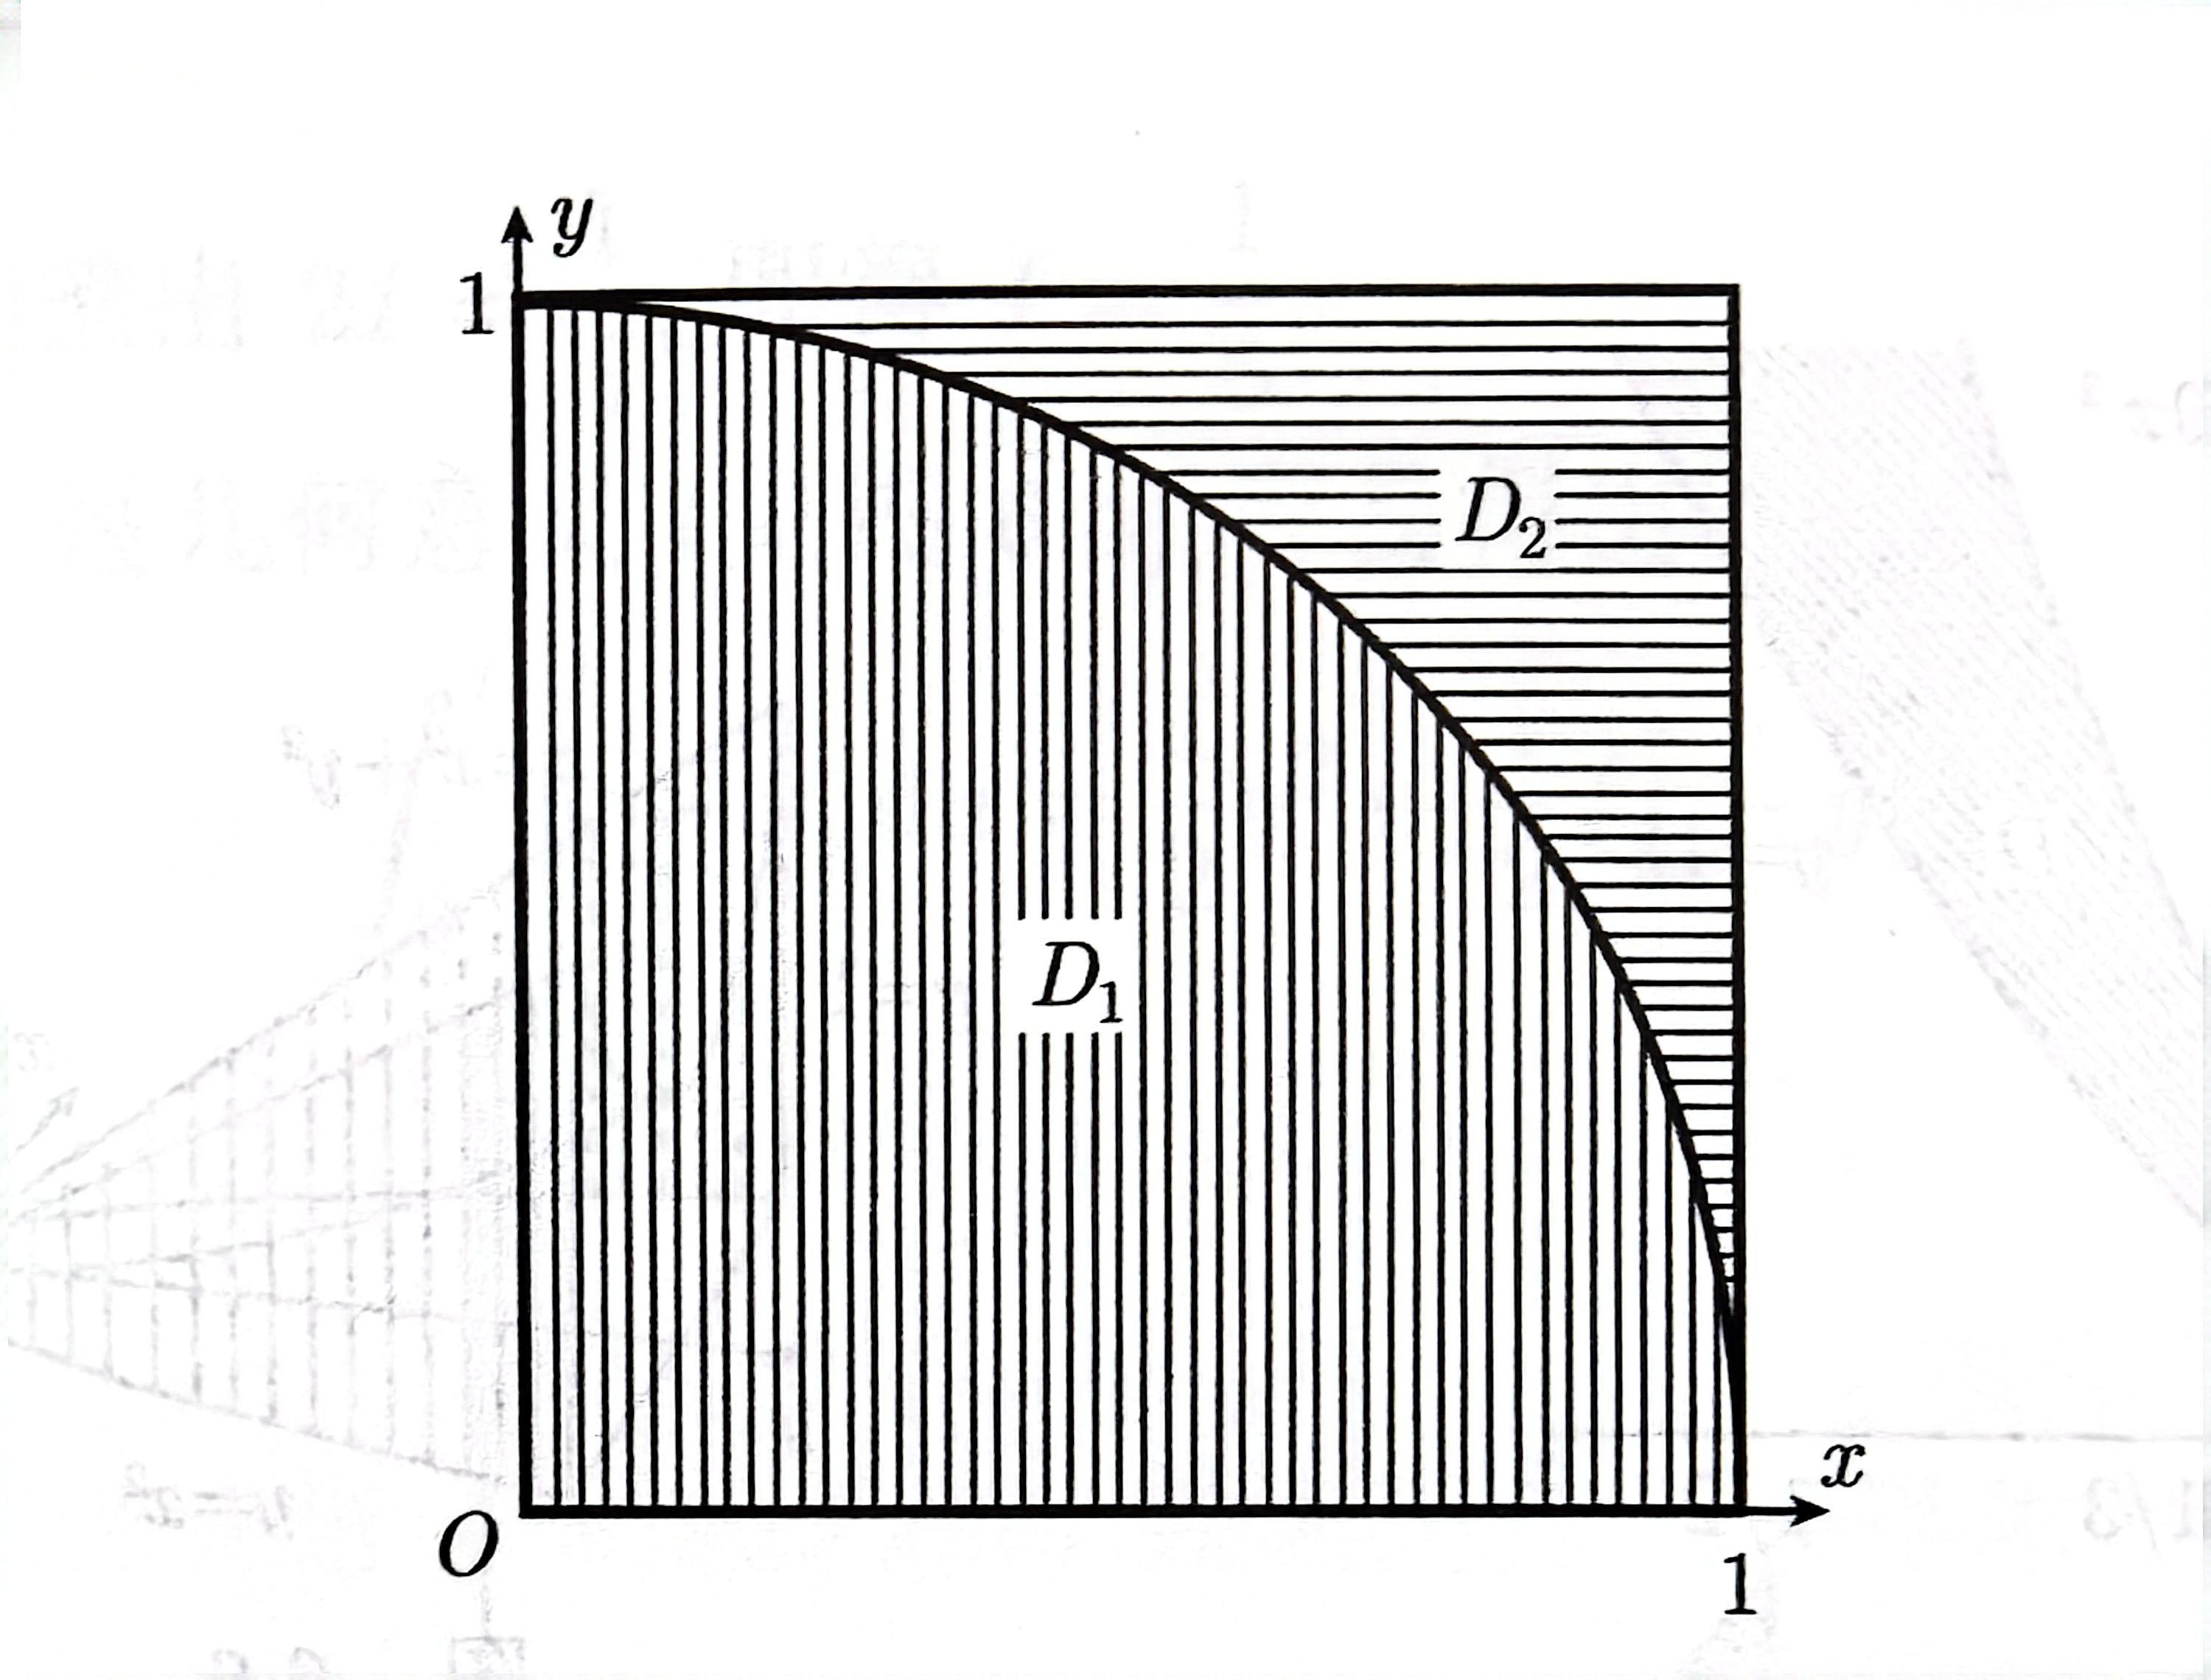
\includegraphics[width=0.5\textwidth]{fig7-8.jpg}
    \caption{例\ref{ex:ch07-13}积分区域}
\end{figure}\par

\subsubsection{积分区域的表示}

本节讨论二重积分转化为累次积分时，如何通过积分区域决定积分上下限.
一般情况下，我们需要画出积分区域的几何图形来帮助确定积分次序和积分上下限.
对于二重积分，积分区域是平面图形，一般都不难画出.
但是仍需要提醒，二重积分转为累次积分时，要求积分下限必须小于积分上限.
这个知识点可以在题目中设置陷阱.

\begin{example}
\label{ex:ch07-14}
计算累次积分
$I = \int _ { - \pi / 2 } ^ { \pi / 2 } \mathrm { ~ d } x \int _ { 0 } ^ { \sin x } \left(  x ^ { 2 }  + y \cos x \right) \sqrt { 1 - y ^ { 2 } } \mathrm { ~ d } y $
\end{example}

\begin{analysis}
设$D_1 = \{(x, y) \mid -\frac{\pi}{2} \le x \le 0, \, \sin x \le y \le 0\}$，
$D_2 = \{(x, y) \mid 0 \le x \le \frac{\pi}{2}, \, 0 \le y \le \sin x\}$.
常犯的错误是认为这个累次积分等于在$D_1 \cup D_2$上的二重积分.
但是，当$-\frac{\pi}{2} < x < 0$时，$\sin x < 0$，
所以在该区间上，累次积分实际上取到了$D_1$上二重积分的负值.
因此，在利用$D_1$与$D_2$的中心对称性时需注意：当$D_1$和$D_2$上的二重积分值相同时，
在题目的累次积分中反而会相互抵消.
\end{analysis}

\begin{solution}
记$f(x,y) = x^2 \sqrt{1-y^2}$，$g(x,y) = y \cos x \sqrt{1-y^2}$.
则：
\begin{eq1}
    I = \iint_{D_2} f(x,y)+g(x,y) ~\d x \d y - \iint_{D_1} f(x,y)+g(x,y) ~\d x \d y
\end{eq1}

注意到$f(x,y) = f(-x,-y)$，$g(x,y) = -g(-x,-y)$.
$D_1$与$D_2$关于原点中心对称.
故：
\begin{eq1}
    \iint_{D_1} f(x,y) ~\d x \d y = \iint_{D_2} f(x,y) ~\d x \d y \\
    \iint_{D_1} g(x,y) ~\d x \d y = -\iint_{D_2} g(x,y) ~\d x \d y
\end{eq1}

则累次积分：
\begin{eq1}
    I &= 2 \iint_{D_2} g(x,y) ~\d x \d y \\
    &= 2 \int_0^{\pi / 2} \d x \int_0^{\sin x} y \cos x \sqrt{1-y^2} ~\d y \\
    &\xlongequal{u = y^2} \int_0^{\pi / 2} \d x \int_0^{\sin^2 x} \cos x \sqrt{1 - u} ~\d u \\
    &= -\frac{2}{3} \int_0^{\pi / 2} \cos x \left[\left( 1-u \right)^{3/2} \bigg|_{0}^{\sin^2 x}\right] ~\d x \\
    &= -\frac{2}{3} \int_0^{\pi / 2} \left( \cos^4 x - \cos x \right) ~\d x \\
    &= -\frac{2}{3} \left( \frac{3!!}{4!!} \cdot \frac{\pi}{2} - 1 \right) ~~~~~\text{（点火公式）}\\
    &= \frac{2}{3} - \frac{\pi}{8}
\end{eq1}
\end{solution}

三重积分的区域往往是几张曲面围成的立体图形.
在画图的时候，不用执着于画出这些“面”本身，
最简单的方法是确定一些顶点和交线的位置，将它们连起来就能自然形成一个立体图.
另外，我们画图的目的是帮助自己选择合适的积分次序，因此我们只需要画出大致图形即可.
有些交线是比较难画的空间曲线，则没有必要画准确.
因为在决定了积分次序之后，我们可能只需要研究它在坐标平面上的投影.\par
~\par

\setstretch{2}

\begin{example}
\label{ex:ch07-15}
计算三重积分：I = $\iiint_{\Omega} \frac{1}{\sqrt{x^2 + y^2}} ~\d V$.
其中$\Omega$是由锥面$z = a -\sqrt{x^2 + y^2}~(a>0)$，
平面$x=0$，$y=0$，$z=x$围成的立体图形.

\setstretch{1.75}
\end{example}

\begin{solution}
四张曲面两两相交，形成$6$条交线.
其中除了锥面与$z=x$的交线是曲线之外，其余$5$条都是直线，可以轻松画出.
由这$5$条线确定$\Omega$的$4$个顶点，也就确定了大致形状（图9）.\par

\begin{figure}[H]
    \centering
    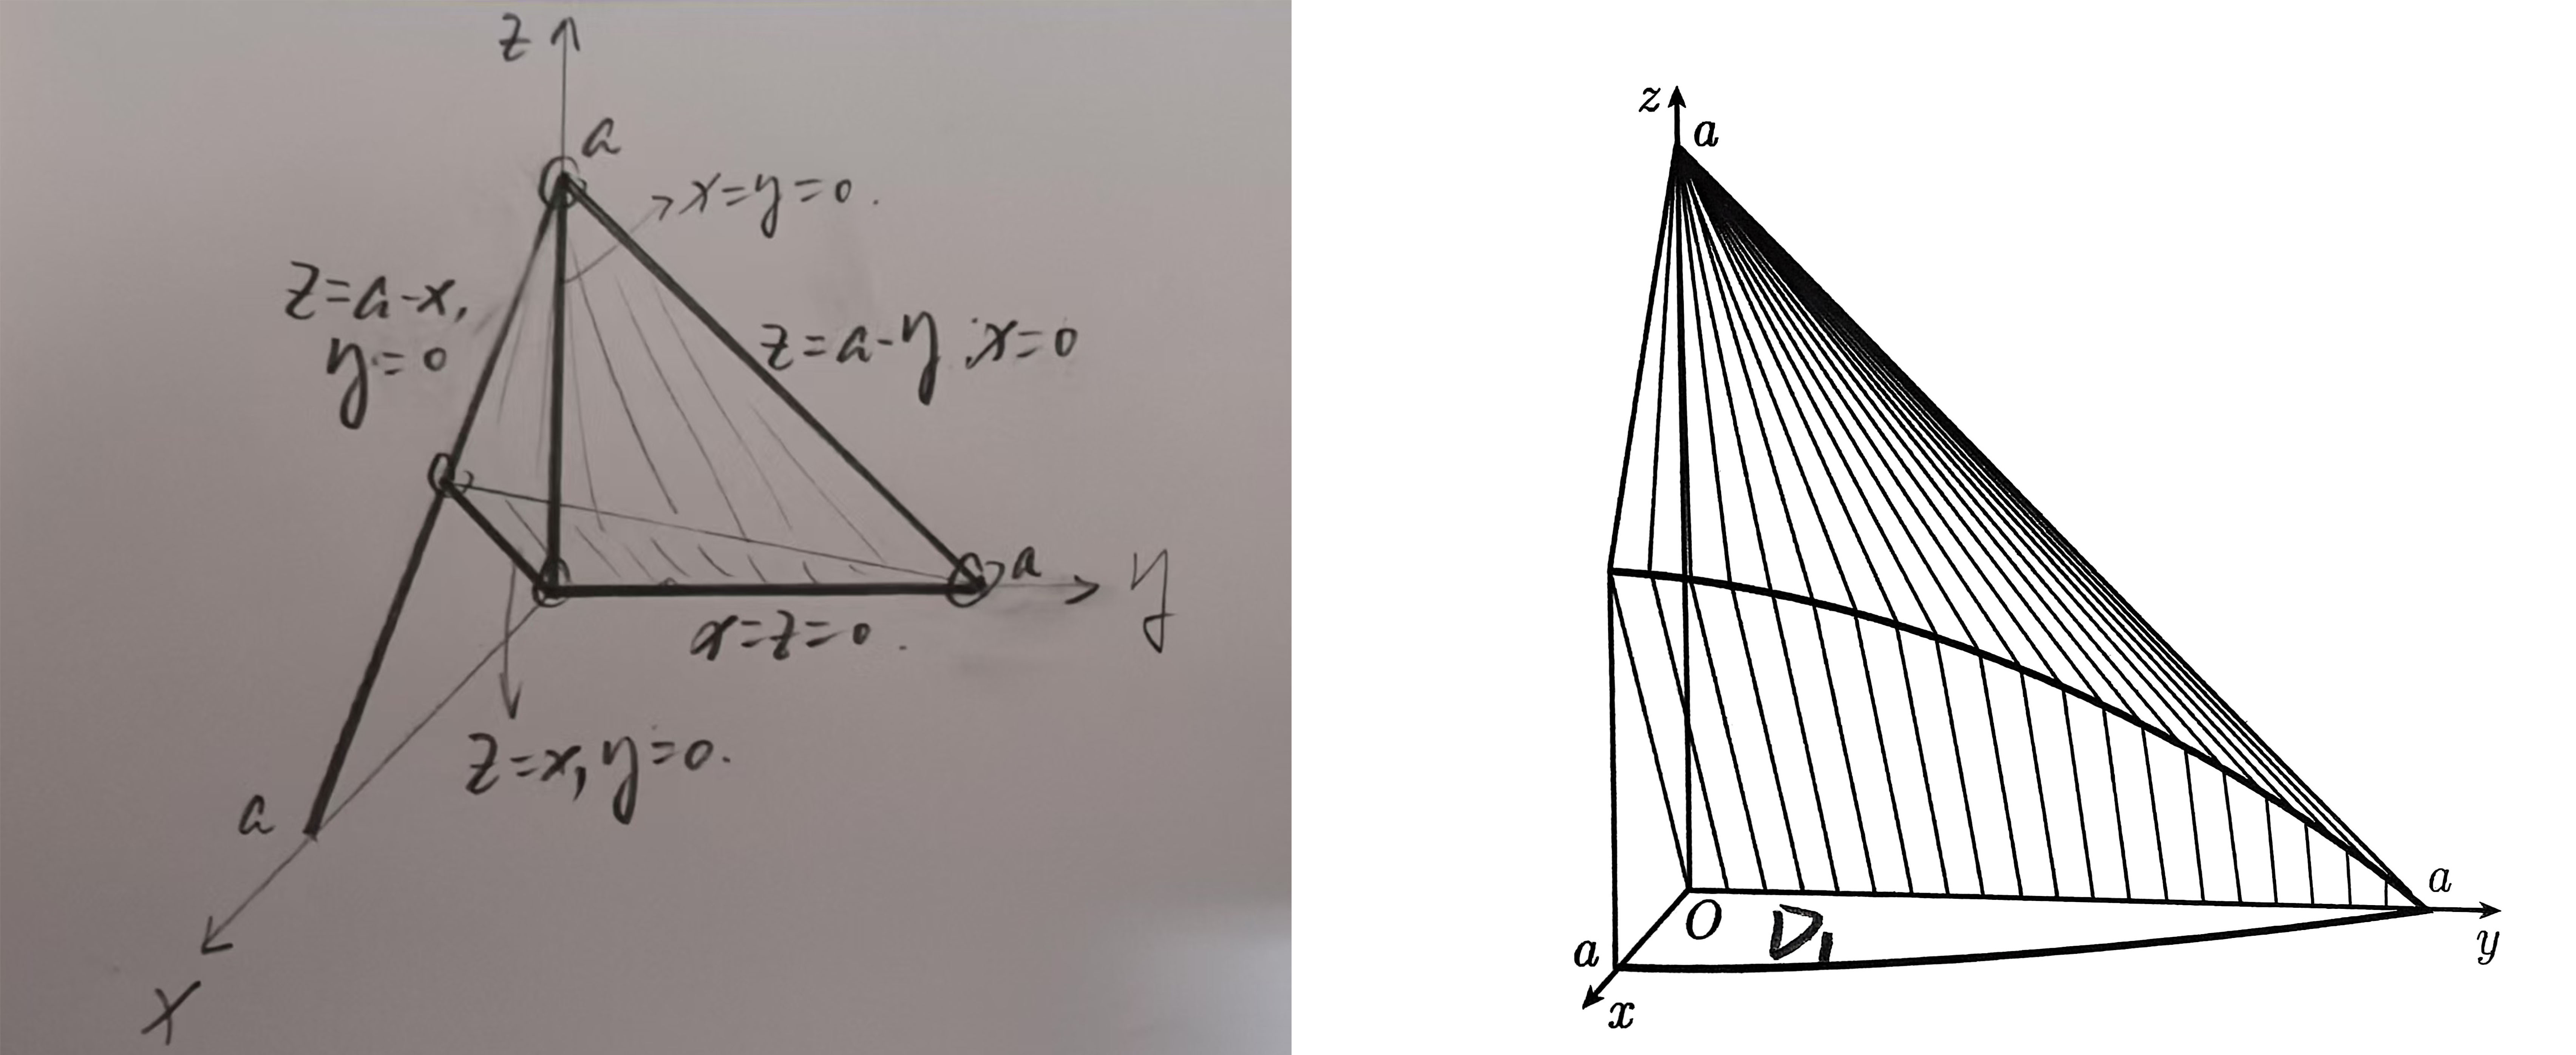
\includegraphics[width=1\textwidth]{fig7-9.jpg}
    \caption{例\ref{ex:ch07-15}草图（左）与标准图（右）}
\end{figure}\par

根据这张图，我们选择把$\Omega$投影到$xOy$平面上，投影区域记为$D$，
而后采取“先一后二”的策略，即先对$z$积分，再在$D_1$上二重积分.
我们只需要把$D_1$的形状描述准确即可.
联立锥面方程与$z=x$，消去$z$，可知围成$D_1$的曲线方程为$x = a -\sqrt{x^2 + y^2}$.

考虑到被积函数和$D_1$的形式，采用柱坐标换元$x = r \cos \theta$，$y = r \sin \theta$.
其中$\theta \in [0,\frac{\pi}{2}]$.
而将曲线方程转化为极坐标方程：
\begin{eq1}
    r \cos \theta = a -r \Rightarrow r = \frac{a}{1 + \cos \theta}
\end{eq1}

则有：
\begin{align*}
    I &= \iint_{D_1} ~\d x \d y \int_{x}^{a - \sqrt{x^2 + y^2}}  \frac{1}{\sqrt{x^2 + y^2}} ~\d z \\
    &= \iint_{D_1'} ~\d r \d \theta \int_{r \cos \theta}^{a-r} \frac{1}{r} \cdot r ~\d z \\
    &= \int_{0}^{\pi / 2} \d \theta \int_{0}^{a / (1 + \cos \theta)} [a - r(1+\cos \theta)] ~\d r\\
    &= \frac{a^2}{2} \int_{0}^{\pi / 2}  \frac{1}{1 + \cos \theta} ~\d \theta\\
    &= \frac{a^2}{2} \int_{0}^{\pi / 2} \frac{\sec^2 \frac{\theta}{2}}{2} ~\d \theta \\
    &=  \frac{a^2}{2} \tan \frac{\theta}{2} \bigg|_{0}^{\pi / 2} \\
    &= \frac{a^2}{2}
\end{align*}
\end{solution}

若积分区域具有对称性，可以只画其中一半.
这样做的好处是，对称面可以作为辅助画图的“脚手架”.

\begin{example}
\label{ex:ch07-16}
求由柱面 $x ^ { 2 } + y ^ { 2 } = a ^ { 2 } , y ^ { 2 } + z ^ { 2 } = a ^ { 2 } , z ^ { 2 } + x ^ { 2 } = a ^ { 2 }$ 所围
区域$\Omega$的体积.
\end{example}

\begin{solution}
显然$\Omega$在$8$个象限内对称，因此只考虑它在第一象限的部分$\Omega_1$.
在画图时，先画出三个柱面与$z=0$，$x=0$和$y=0$的交线.
这其实就有了$\Omega$的框架.
要补全这个图形只需要知道剩下一个顶点的位置.
这是容易确定的.
联立三个柱面方程可知顶点的坐标$x=y=z=\frac{a}{\sqrt{2}}$.
连接各顶点画出$\Omega_1$的草图（图10）.

\begin{figure}[H]
    \centering
    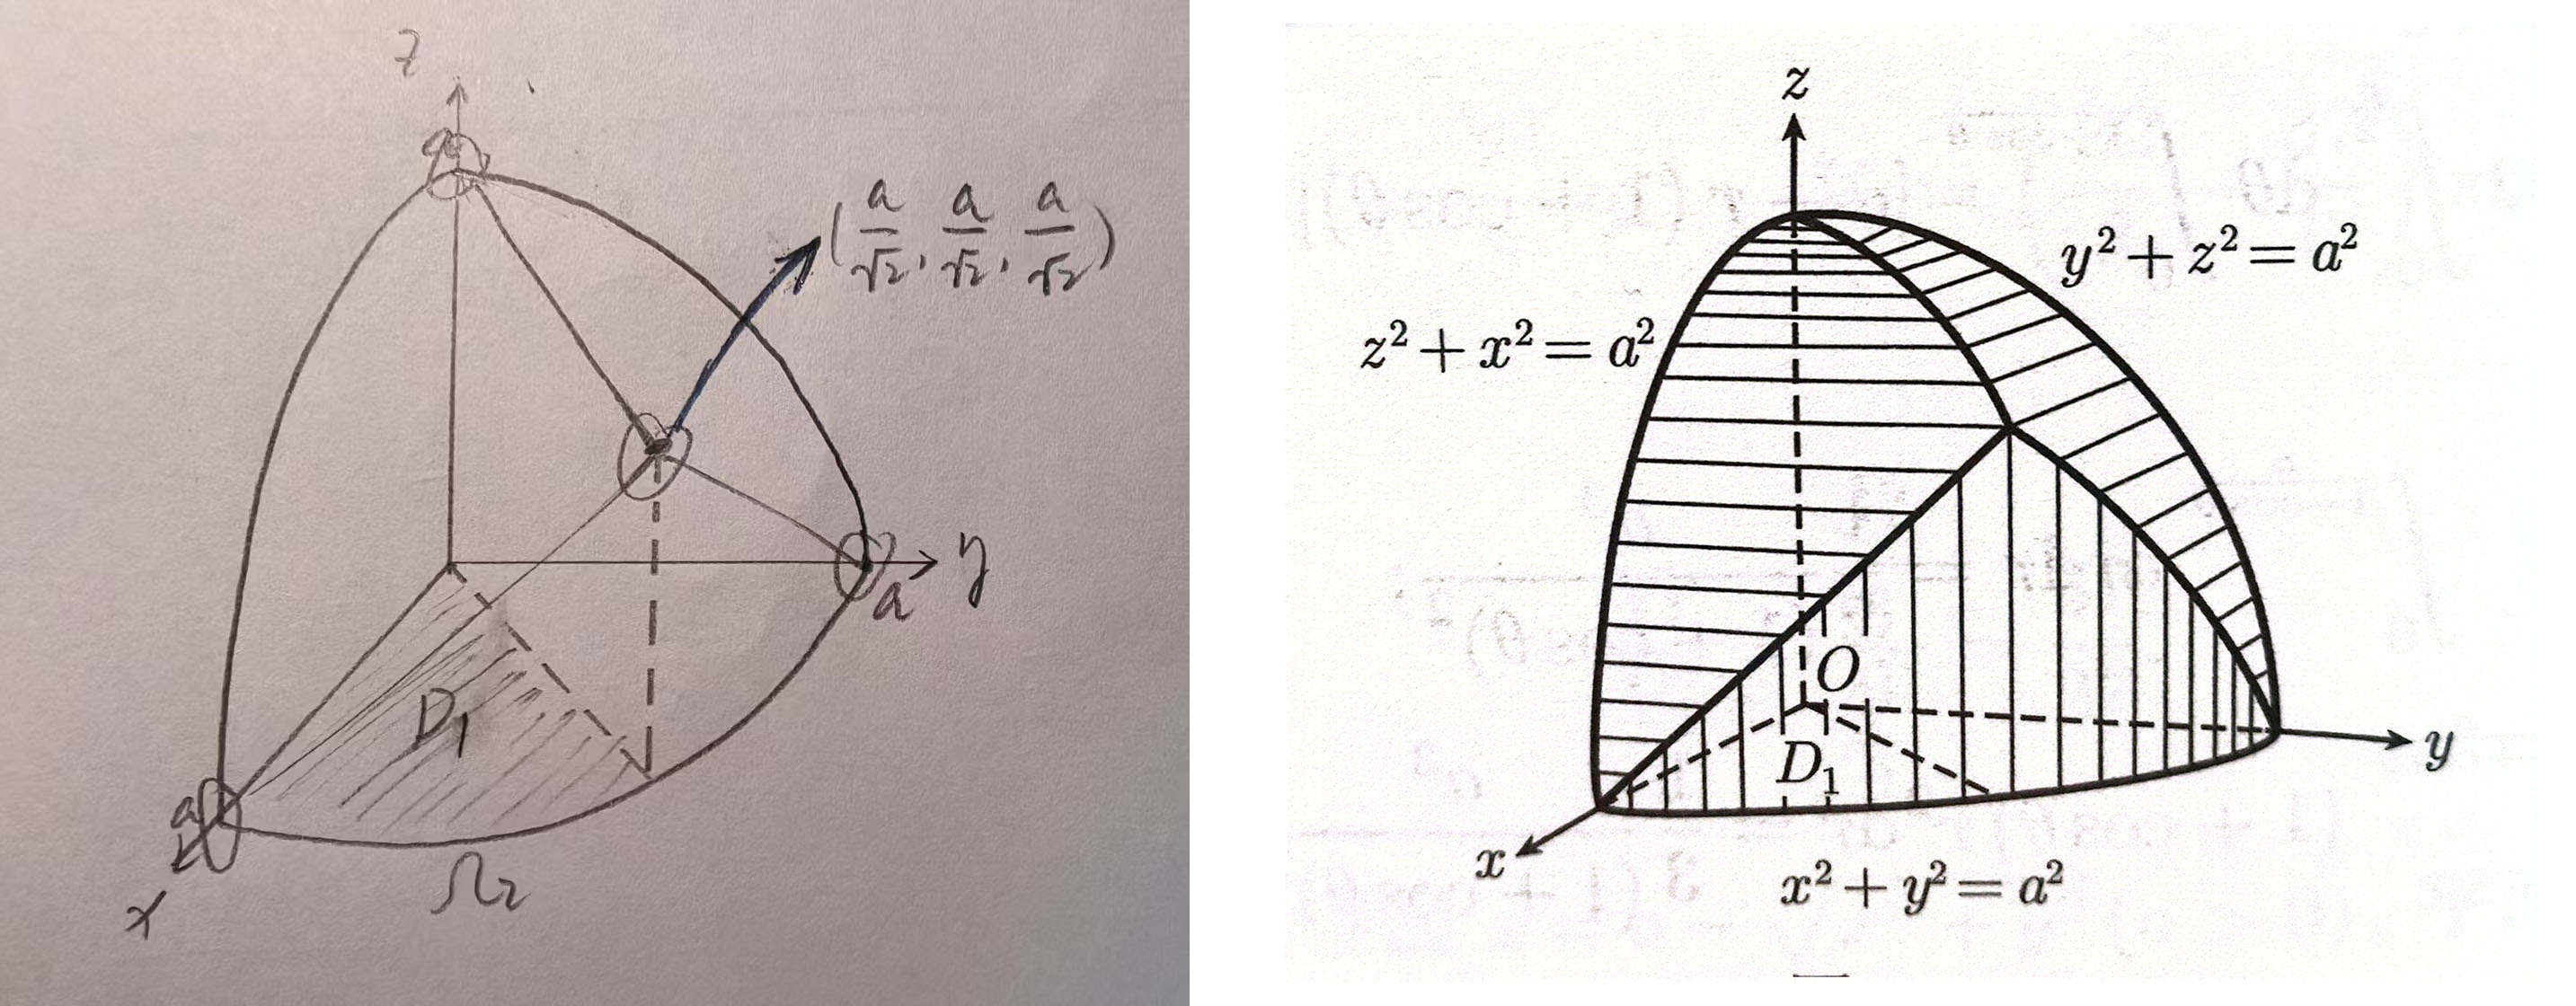
\includegraphics[width=1\textwidth]{fig7-10.jpg}
    \caption{例\ref{ex:ch07-16}草图（左）与标准图（右）}
\end{figure}

我们发现还是很难直接转化成累次积分.
原因是我们还有对称性没有使用：
在画图时容易发现，$\Omega_1$关于$x=y$，$y=z$，$x=z$平面都是对称的.
我们只需要取其中之一，例如用$x=y$将$\Omega_1$切成两半，其中一半记为$\Omega_2$，就可以在投影区域$D_1$上通过二重积分计算体积了.
注意$\Omega_2$的体积是$\Omega$的$\frac{1}{16}$.
故：
\begin{eq1}
    \frac{V}{16} = \iint_{D_1} ~\d x \d y \int_{0}^{\sqrt{a^2 - x^2}} ~\d z
    = \iint_{D_1} \sqrt{a^2 - x^2} ~\d x \d y
\end{eq1}

由于$D_1$是扇形区域，采用极坐标变换：
\begin{eq1}
    \frac{V}{16}
    &= \int_{0}^{\pi / 4} ~\d \theta \int_{0}^{a} \sqrt{a^2 - r^2 \cos^2 \theta } \cdot r ~\d r \\
    &\xlongequal{u = r^2} \frac{1}{2} \int_{0}^{\pi / 4} ~\d \theta \int_{0}^{a^2} \sqrt{a^2 - u \cos^2 \theta} ~\d u \\
    &= \frac{1}{2} \int_{0}^{\pi / 4} \frac{-2}{3 \cos^2 \theta} \left( a^2 - u \cos^2 \theta \right)^{3/2} \bigg|_{0}^{a^2} ~\d \theta \\
    &= \frac{a^2}{3} \int_{0}^{\pi / 4} \frac{1 - \sin^3 \theta}{\cos^2 \theta} ~\d \theta \\
    &= \frac{a^2}{3} \left[ 1 - \left( \frac{3\sqrt{2}}{2} -2 \right) \right] \\
    &= \frac{(2-\sqrt{2}) a^3}{2}
\end{eq1}

即$V = 8(2-\sqrt{2}) a^3$.
\end{solution}

\subsubsection{积分次序}

如果累次积分的顺序选择得不好，不仅会增加计算难度，有时甚至做不出来.
因此需慎重抉择积分次序.
有时题目会故意给出次序不合理的累次积分，需要根据积分上下限画出对应积分区域的图像，
交换积分的次序.
这就要求同学们对积分的难易程度（包括是否可解）有所把握.

\begin{example}
\label{ex:ch07-17}
计算积分：
$\int_{-1}^{1} \d x \int_{-1}^{x} \frac{x}{\sqrt{1-x^2 + y^2}} ~\d y$.
\end{example}

\begin{solution}
交换积分次序：
\begin{eq1}
    \int_{-1}^{1} \d x \int_{-1}^{x} \frac{x}{\sqrt{1-x^2 + y^2}} ~\d y
    &=
    \int_{-1}^{1} \mathrm{d} y \int_{y}^{1} \frac{x}{\sqrt{1-x^2 + y^2}} ~\mathrm{d} x \\
    &= -\int_{-1}^{1} \sqrt{1-x^2 +y^2} \bigg|_{x=y}^{x=1} ~\d y \\
    &= \int_{-1}^{1} (1 - |y|) ~\d y \\
    &= 2 \int_{-1}^{1} (1-y) ~\d y = 1
\end{eq1}
\end{solution}

\begin{example}[2023]
\label{ex:ch07-18}
计算积分
$I = \iint _ { D } \left( \frac { 3 x ^ { 2 } \sin y } { y } + 2e^{x^2}\right) \mathrm { d } \sigma ,$
其中 $D$ 由 $y = x$ ，$y = x ^ { 3 }$ 围成.
\end{example}

\begin{analysis}
这道题如果先对$x$积分，则$e^{x^2}$是积不出来的；
若先对$y$积分，则$\frac{\sin y}{y}$又积不出来.
所以我们要把这积分的两个项拆分开，按各自合适的积分次序来解决.
\end{analysis}

\begin{solution}
首先注意积分区域$D$关于原点是中心对称的，
而被积函数满足$f(x,y) = f(-x,-y)$.
故设$D_1 = \{(x, y) \mid 0 \le x \le 1, \, x^3 \le y \le x\}$，
则：
\begin{eq1}
    I = 2\iint _ { D_1 } \frac { 3 x ^ { 2 } \sin y } { y } \mathrm { d } \sigma
    + 2\iint _ { D_1 }   2 e^{x^2} \mathrm { d } \sigma
\end{eq1}

对于前一个积分，应先对$x$积分，即：
\begin{eq1}
    \iint _ { D_1 } \frac { 3 x ^ { 2 } \sin y } { y } ~\mathrm { d } \sigma
    &= \int_{0}^{1} \d y \int_{y}^{\sqrt[3]{y}} \frac{3x^2 \sin y}{y} \, \mathrm{d}x \\
    &= \int_0^1 ~ \frac{\sin y}{y} x^3 \bigg|_{x=y}^{x=\sqrt[3]{y}} ~\d y \\
    &= \int_0^1 \left( \sin y - y^2 \sin y \right) ~\d y \\
    &= 3 - 2 \sin 1 - 2 \cos 1
\end{eq1}

对于后一个积分，应先对$y$积分，即：
\begin{eq1}
    \iint _ { D_1 }   2 e^{x^2} \mathrm { d } \sigma
    &= \int_{0}^{1} \d x \int_{x}^{x^3} 2 e^{x^2} \mathrm{d} y \\
    &= \int_0^1 2(x^3 - x) e^{x^2} ~\d x \\
    &\xlongequal{u = x^2} \int_0^1 (u-1)e^u ~\d u \\
    &=  2-e
\end{eq1}

最终得到：
\begin{eq1}
    I = 2\cdot (3 - 2 \sin 1 - 2 \cos 1) + 2 \cdot (2-e) = 5 - 4 \sin 1 - 4 \cos 1 - 2e
\end{eq1}
\end{solution}

\subsubsection{*利用重积分计算一元函数定积分}

\begin{example}
\label{ex:ch07-19}
计算Gauss积分：
$\int_{-\infty}^{\infty} e^{-x^2} ~\d x = \sqrt{\pi}$.
\end{example}

\begin{solution}
记该积分为$I$.
可用两个$I$组合出一个二重积分：
\begin{eq1}
    I^2 &=
    \int_{-\infty}^{+\infty} e^{-x^2} ~\d x \cdot
    \int_{-\infty}^{+\infty} e^{-y^2} ~\d y \\
    &= \iint_{\mathbb{R}^2} e^{-(x^2 + y^2)} ~\d x \d y
\end{eq1}

采用极坐标变换：
\begin{eq1}
    I^2 &= \int_{0}^{2 \pi} ~\d \theta \int_{0}^{+\infty} e^{-r^2} \cdot r ~\d r \\
    &\xlongequal{u = r^2} 2\pi \int_{0}^{+\infty} \frac{e^{-u}}{2} ~\d u \\
    &= \pi \left( -e^{-u} \right)\bigg|_{0}^{+\infty} \\
    &= \pi
\end{eq1}
\end{solution}

\begin{example}
\label{ex:ch07-20}
计算：
$\int_{0}^{+\infty} \frac{\arctan{\pi x} - \arctan x}{x} ~\d x$.
\end{example}

\begin{solution}
观察到被积函数的形式可以逆用牛顿莱布尼茨公式（此时将$x$视为参数，引入另一积分变量$y$）：
\begin{eq1}
    \arctan{\pi x} - \arctan x
    =
    \arctan{xy}\bigg|_{1}^{\pi}
    =
    \int_{1}^{\pi} \frac{x}{1+(xy)^2} ~\d y
\end{eq1}

则原积分化为二重积分，可以交换积分次序：
\begin{eq1}
    \int_{0}^{+\infty} \frac{\arctan{\pi x} - \arctan x}{x} ~\d x &=
    \int_{0}^{+\infty} ~\d x \int_{1}^{\pi} \frac{1}{1+(xy)^2} ~\d y \\
    &= \int_{1}^{\pi} ~\d y \int_{0}^{+\infty} \frac{1}{1+(xy)^2} ~\d x \\
    &= \int_{1}^{\pi} \frac{1}{y} \left(\arctan xy \bigg|_{0}^{+\infty} \right)  ~\d y \\
    &= \frac{\pi}{2} \int_{1}^{\pi} \frac{1}{y} ~\d y \\
    &= \frac{\pi}{2} \ln \pi
\end{eq1}
\end{solution}

\begin{example}
\label{ex:ch07-21}
计算Dirichlet积分：
$\int_{0}^{+\infty} \frac{\sin x}{x} ~\d x = \frac{\pi}{2}$.
\end{example}

\begin{solution}
方法类似上例，通过逆用牛顿莱布尼茨公式引入另一积分变量$y$，使之转化为二重积分：
\begin{eq1}
    \frac{1}{x} = - \frac{e^{-xy}}{x}\bigg|_{0}^{+\infty} = \int_{0}^{+\infty} e^{-xy} ~\d y
\end{eq1}

则原积分：
\begin{eq1}
    \int_{0}^{+\infty} \frac{\sin x}{x} ~\d x
    &= \int_{0}^{+\infty} ~\d x \int_{0}^{+\infty} e^{-xy} \sin x ~\d y \\
    &= \int_{0}^{+\infty} \left( \int_{0}^{+\infty} e^{-xy} \sin x  ~\d x  \right) ~\d y
\end{eq1}

我们将内层积分记为$I$.
对积分技巧熟悉的同学可以看出，这个积分应该通过两次分部积分来计算：
\begin{eq1}
    I &= -\int_{0}^{+\infty} e^{-xy} \d \cos x \\
    &= -\left( e^{-xy} \cos x \right) \bigg|_{0}^{+\infty}
    - \int_{0}^{+\infty} ye^{-xy}  ~\d \sin x \\
    &= 1 -\left(y  e^{-xy} \sin x \right) \bigg|_{0}^{+\infty} - y^2 \int_{0}^{+\infty} e^{-xy} \sin x ~\d x   \\
    &= 1 - y^2 I
\end{eq1}

可知$I = \frac{1}{y^2 + 1}$.
则原积分化为：
\begin{eq1}
    \int_{0}^{+\infty} \frac{\sin x}{x} ~\d x
    &= \int_{0}^{+\infty} \frac{1}{y^2 + 1} ~\d y \\
    &= \left( \arctan y \right) \bigg|_{0}^{+\infty} \\
    &= \frac{\pi}{2}
\end{eq1}
\end{solution}

\begin{example}
\label{ex:ch07-22}
计算Fresnel积分：$\int_{-\infty}^{+\infty} \sin (x^2) ~\d x$.
\end{example}

\begin{solution}
令$t = x^2$，则：
\begin{eq1}
    \int_{-\infty}^{+\infty} \sin (x^2) ~\d x
    = 2 \int_{0}^{+\infty} \frac{\sin t}{2 \sqrt{t}} ~\d t
    = \int_{0}^{+\infty} \frac{\sin t}{\sqrt{t}} ~\d t
\end{eq1}

这里原本可以仿照上例的方法，利用指数函数的积分处理分母上的$\sqrt{t}$.
但是尝试过后发现行不通.
这里需要借用Gauss积分的结论. 我们知道：
\begin{eq1}
    \int_{0}^{+\infty} e^{-x^2} ~\d x
    = \frac{1}{2}\int_{-\infty}^{\infty} e^{-x^2} ~\d x
    = \frac{\sqrt{\pi}}{2}
\end{eq1}

则通过换元法可知：
\begin{eq1}
    \frac{1}{\sqrt{t}} = \frac{2}{\sqrt{\pi}} \int_{0}^{+\infty} e^{-ty^2} ~\d y
\end{eq1}

将其代入原积分，将其变为二重积分：
\begin{eq1}
    \int_{0}^{+\infty} \frac{\sin t}{\sqrt{t}}~ \d t
    &= \frac{2}{\sqrt{\pi}} \int_{0}^{+\infty} \d t \int_{0}^{+\infty} e^{-ty^2} \sin t ~\d y \\
    &= \frac{2}{\sqrt{\pi}} \int_{0}^{+\infty} \d y \int_{0}^{+\infty} e^{-ty^2} \sin t ~\d t
\end{eq1}

内层积分的算法与上例中计算$I$的方法完全相同，只不过把$y$换成了$y^2$.
这里不再写一遍计算过程.
最终得到：
\begin{eq1}
    \int_{0}^{+\infty} e^{-ty^2} \sin t = \frac{1}{1+y^4}
\end{eq1}

因此原积分化为：
\begin{eq1}
    \int_{-\infty}^{+\infty} \sin (x^2) ~\d x
    = \frac{2}{\sqrt{\pi}} \int_{0}^{+\infty} \frac{1}{1+y^4}~\d y
\end{eq1}

我们曾经在第三章讲义中介绍过这个积分的计算方法，这里也不再展示.
最终得到：
\begin{eq1}
    \int_{-\infty}^{+\infty} \sin (x^2) ~\d x &=
    \frac{2}{\sqrt{\pi}} \left(\frac { 1 } { 4 \sqrt { 2 } } \ln \frac { x ^ { 2 } + \sqrt { 2 } x + 1 } { x ^ { 2 } - \sqrt { 2 } x + 1 } +
    \frac { 1 } { 2 \sqrt { 2 } } \arctan \frac { x ^ { 2 } - 1 } { \sqrt { 2 } x } \right)\bigg|_{0}^{+\infty} \\
    &= \frac{2}{\sqrt{\pi}} \cdot \frac{\pi}{2\sqrt{2}} = \sqrt{\frac{\pi}{2}}
\end{eq1}
\end{solution}

\subsubsection{*与二重积分有关的极限计算}

\begin{example}
\label{ex:ch07-23}
计算$\lim\limits_{n \to \infty} \sum_{i=1}^{n} \sum_{j=1}^{n} \frac{1}{(n+i)\sqrt{n^2 + j^2}}$
\end{example}

\begin{analysis}
利用二重积分的定义.
\end{analysis}

\begin{solution}
\begin{eq1}
    \lim\limits_{n \to \infty} \sum_{i=1}^{n} \sum_{j=1}^{n} \frac{1}{(n+i)\sqrt{n^2 + j^2}}
    &= \lim\limits_{n \to \infty} \sum_{i=1}^{n} \sum_{j=1}^{n} \frac{1}{n^2} \cdot \frac{1}{\left(1 + \dfrac{i}{n} \right) \sqrt{1 + \left( \dfrac{j}{n} \right)^2}} \\
    &= \iint_{D} \frac{1}{(1+x)\sqrt{1 + y^2}}~\d x \d y \\
    &= \int_{0}^{1} \frac{1}{1+x}~\d x \int_{0}^{1} \frac{1}{\sqrt{1+y^2}}~\d y \\
    &= \ln (1+x) \bigg|_{0}^{1} \cdot \ln (y + \sqrt{1+y^2}) \bigg|_{0}^{1} \\
    &= \ln 2 \cdot \ln (1 + \sqrt{2})
\end{eq1}
\end{solution}

\begin{example}
\label{ex:ch07-24}
设区域$D_r = \left\{ (x,y) \mid x^2 + y^2 \le r^2 \right\}~(r > 0)$.计算下列极限的值：
\begin{eq1}
    \lim\limits_{r \to 0^{+}} \frac{\displaystyle\iint_{D_r} e^{x^2 + y^2} \cos (x^2 + y^2) ~\d \sigma}{r^2}
\end{eq1}
\end{example}

\begin{solution}[解法一]
分子上的二重积分可以看成关于$r$的一元函数$f(r)$.
只需要算出它的表达式即可.
采用极坐标换元$x = \rho \cos \theta$，$y = \rho \sin \theta$：
\begin{eq1}
    \iint_{D_r} e^{x^2 + y^2} \cos (x^2 + y^2) ~\d \sigma
    &= \int_{0}^{2\pi} \d \theta \int_{0}^{r} e^{\rho^2} \cos (\rho^2) \rho ~\d \rho \\
    &= 2 \pi \int_{0}^{r} e^{\rho^2} \cos (\rho^2) \rho ~\d \rho
\end{eq1}

可以继续计算出这个积分关于$r$的表达式，但是这样有些麻烦.
注意到这个积分是关于$r$的变上限积分，可以使用洛必达法则：
\begin{eq1}
    \lim\limits_{r \to 0^{+}} \frac{\displaystyle\iint_{D_r} e^{x^2 + y^2} \cos (x^2 + y^2) ~\d \sigma}{r^2}
    &= \lim\limits_{r \to 0^{+}} \frac{2 \pi \displaystyle \int_{0}^{r} e^{\rho^2} \cos (\rho^2) \rho ~\d \rho}{r^2} \\
    &= \lim\limits_{r \to 0^{+}} \frac{2\pi e^{r^2} \cos (r^2) \cdot r}{2r} \\
    &= \pi \lim\limits_{r \to 0^{+}} e^{r^2} \cos (r^2) \\
    &= \pi
\end{eq1}
\end{solution}

\begin{solution}[解法二]
上述解答启发我们，由于$D_r$无限收缩，极限最终只取决于被积函数在原点处的取值.
这一点可以用积分中值定理描述. 由积分区域面积$S(D_r) = \pi r^2$，可知存在$(\xi_r, \eta_r) \in D_r$，使得：
\begin{eq1}
    \iint_{D_r} e^{x^2 + y^2} \cos (x^2 + y^2) ~\d \sigma
    = \pi r^2 \cdot e^{\xi_r^2 + \eta_r^2} \cos (\xi_r^2 + \eta_r^2)
\end{eq1}

当$r \to 0^{+}$时，$(\xi_r , \eta_r) \to (0,0)$.
故极限值：
\begin{eq1}
    \lim\limits_{r \to 0^{+}} \frac{\displaystyle\iint_{D_r} e^{x^2 + y^2} \cos (x^2 + y^2) ~\d \sigma}{r^2}
    &= \lim\limits_{r \to 0^{+}} \frac{\pi r^2 \cdot e^{\xi_r^2 + \eta_r^2} \cos (\xi_r^2 + \eta_r^2)}{r^2} \\
    &= \pi \cdot e^0 \cos 0 = \pi
\end{eq1}
\end{solution}
